\documentclass{article}
%\usepackage{arxiv}
\usepackage[utf8]{inputenc}
\usepackage[english]{babel}
\usepackage{amssymb, amsmath, amsthm, amsfonts}
\usepackage{thmtools, mathtools, mathrsfs, dsfont}
\usepackage{bbm}
\usepackage[square,numbers]{natbib}
\bibliographystyle{abbrvnat}
\usepackage{algorithm}
\usepackage{algpseudocode}
\usepackage{forloop}
\usepackage[pdftex]{graphicx}  %remove demo option in your document
\usepackage{sidecap}

\graphicspath{{figures}}

\newtheorem{theorem}{Theorem}
\newtheorem{proposition}{Proposition}
\newtheorem{lemma}{Lemma}
\newtheorem{corollary}{Corollary}[theorem]
\theoremstyle{definition}
\newtheorem{definition}{Definition}
\theoremstyle{remark}
\newtheorem{remark}{Remark}

\newcommand{\reals}{\mathbb{R}}
\newcommand{\sep}{\operatorname{sep}}
\newcommand{\cl}{\operatorname{cl}}
\newcommand{\vol}{\operatorname{vol}}
\newcommand{\boa}{\operatorname{BoA}}
\newcommand{\mcN}{\mathcal{N}}
\newcommand{\mcK}{\mathcal{K}}
\newcommand{\mcU}{\mathcal{U}}
\newcommand{\mcX}{\mathcal{X}}
\newcommand{\T}{\operatorname{T}}
\newcommand{\TR}{\T\!\mathbb{R}}
\newcommand{\TM}{\T\!M}
\newcommand{\TpM}{\T_p\!M}
\newcommand{\Diffeo}{\operatorname{Diffeo}}
\newcommand{\Hpert}{H^{\text{pert}}}
\newcommand{\inv}{\operatorname{Inv}}

\newcommand{\defvec}[1]{\expandafter\newcommand\csname v#1\endcsname{{\mathbf{#1}}}}
\newcommand{\dm}[1]{\ensuremath{\mathrm{d}{#1}}} % dx dy dz dmu
\newcounter{ct}
\forLoop{1}{26}{ct}{
    \edef\letter{\alph{ct}}
    \expandafter\defvec\letter
}

% captial \vA
\forLoop{1}{26}{ct}{
    \edef\letter{\Alph{ct}}
    \expandafter\defvec\letter
}

%\title{Finally, an \emph{actual} universal approximation result for multi-stable dynamical systems}
%\title{RNNs can approximate multistable dynamical systems on an infinite time horizon}
\title{Universal approximation of multistable dynamical systems on an infinite time horizon by RNNs}
\author{\'Abel S\'agodi and Il Memming Park}
\date{\today}



\begin{document}
\maketitle

\section*{Abstract}

\section{Introduction}
The versatility or flexibility of a given machine learning paradigm is usually established by proving its universality.
We say that a family of transformations is universal when its elements can approximate as accurately as one wants all the elements of a sufficiently rich class containing, for example, all continuous or even all measurable transformations.

%Modeling/Reconstructing dynamics examples. mention?
%gene regulation \citep{paczko2024neural}

Recurrent Neural Networks (RNNs) are believed to be universal approximators.
For example, \citet{durstewitz2023reconstructing} claims that 
%a library of basis functions or
 a neural network may be used to closely approximate the vector field or the trajectories of any given dynamical system.
However, universal approximation results based on vector fields are limited in scope, as the behavior of the ODE they support might deviate from the target.
Existing results about approximating dynamical systems either focus on finite time horizon approximation or on approximating stable dynamical systems on an infinite time horizon.
This misses important behavior of the system (e.g. temporal generalization of the approximation, see Fig.~\ref{fig:lc_period_div}).

A key motivation for extending approximation results to the infinite time horizon lies in its ability to capture qualitative behaviors over time. For example, infinite time horizon approximation allows us to better understand how a system's behavior unfolds over extended periods, providing insights into stability, transitions, and equilibrium states.
 Furthermore, an effective infinite time horizon approximation ensures robustness: small perturbations, such as noise, do not result in abrupt increases in approximation error, but instead produce gradual, smooth deviations in the system's trajectory.
%the second point needs to be worked out: with added noise the error would jump for trajectories at separatrices

%We seek to extend approximation results for dynamical systems to multi-stable systems (systems without chaos) on an infinite time horizon through Neural ODEs (NODEs).
Our work aims to bridge this gap by extending the approximation of dynamical systems to multi-stable systems—those with multiple equilibrium states but no chaotic behavior—over an infinite time horizon. 
To achieve this, we leverage Neural Ordinary Differential Equations (NODEs) as a framework for constructing such approximations.
% By using NODEs, we can model continuous-time dynamical systems while ensuring that key properties, such as stability and smooth error bounds under perturbations, are maintained.
We provide a fist-of-its-kind \textbf{approximation result for multi-stable systems on the infinite time horizon}, laying the groundwork for future advances in both theory and applications of neural approximators in long-term dynamical modeling.

%mention that vanilla RNNs are not universal approximators?
%how we will do this
%outlay of paper


\paragraph{Formulation: lack of theory on time generalization/forecasting}
ANNs can generalize. After learning the data presented to them (a sample), ANNs can often correctly infer the unseen part of a population even if the sample data contain noisy information. As forecasting is performed via prediction of future behavior (the unseen part) from examples of past behavior, it is an ideal application area for neural networks, at least in principle. \citep{zhang1998forecasting}



\section{Approximation of dynamical systems: A vast literature with limited results}
%sota 
Accurately approximating dynamical systems is essential for understanding and predicting complex behaviors across a range of applications, from robotics to climate modeling.
Recent advances in machine learning have enabled data-driven approaches to approximating these systems, providing new ways to model complex dynamics over extended periods.
Here, we review key approaches in the literature and highlight emerging techniques that address these challenges, before we introduce our method that extends to multi-stable and complex systems over infinite time horizons.
%
%For an overview of the literature, see [litrev]
See also \citep{li2022approximation} and \citep{jiang2023brief}.

Density results describe the completeness of a hypothesis class relative to a target class, emphasizing the extent to which the hypothesis class can approximate every element in the target class with arbitrary precision.


%TODO: unify terminology: UAP, density result...
It is important to realize that a class of models (a hypothesis class) can have the universal approximation property (UAP) \emph{for a specific target class} given \emph{a specific metric to compare} (see also Sec.~\ref{sec:approximationtheory}).
This property implies that the hypothesis class is dense in the target class, hence such results are also referred to as \emph{density results}.

\begin{table}[h]
\begin{tabular}{|l|l|l|l|l|l|}
%\hline
\cline{2-6}
    \multicolumn{1}{c|}{}							%leave out size?
 						&  Time interval & FMP	& Finite size 		&  Input     	&     Time   \\\cline{2-6}\hline
\citet{cybenko1989approximation} 	& Finite	& No 	& Yes 			&  Yes		&	Continuous\\\hline  %vf
\citet{funahashi1989approximate} 	& Finite	& No		& Yes			&  Yes		&	Continuous\\\hline  %vf
\citet{hornik1989multilayer} 		& Finite	& No 	& Yes			& Yes		&	Continuous\\\hline  %vf
\citet{funahashi1993approximation} 	& Finite	& No		& Yes			&  Yes		&	Continuous\\\hline
\citet{jin1995approximation}		& Finite	& No		& Yes			& Yes		&	Continuous	\\\hline
\citet{hammer2000approximation}	& Finite     & No 	& Yes			& Yes		& 	Discrete	\\\hline
\citet{jin1995universal}			& Finite	& No		& Yes			& Yes		&	Discrete	\\\hline
\citet{bai2019deq} 				& Infinite	& Yes	& No		 	& Yes 			&	Discrete		\\\hline
\citet{schafer2007uap} 			& Infinite 	& Yes	& No			& Yes 			&	Discrete\\\hline
\citet{wang2024state}			& Infinite   & Yes 	& No 		& Yes			& 	Continuous\\\hline % FMP type: (exp. decay) 
\dots&\dots &\dots&\dots&\dots&\dots\\
\end{tabular}
\end{table}


\paragraph{Learning sequences}
 A critical review of recurrent neural networks for sequence learning \citep{williams1989learning, pearlmutter1989learning, lipton2015rnn}.
 
 %\paragraph{Operators}%approximation of an operator

\subsection{Universal approximation for mappings}\label{sec:uapmappings}
This is the basic ingredient for many of the UAP results in the literature and will be the starting point for our proof.
See for the  Supp.Sec.~\ref{sec:uniapproxffn}.


%vector fields (which is just FNN setting)
\subsection{Approximating vector fields}\label{sec:uapvfs}
 FNNs can approximate smooth functions effectively, making them suitable for approximating vector fields \citep{doya1993universality}.
This is a direct consequence of the UAP of FNNs for mappings, see Supp.Sec.~\ref{sec:uniapproxffn}.



\paragraph{Spiking neural network}
%only approximates vector field 
It is possible to approximate vector fields with other architectures.
For example, in limit $N\rightarrow\infty$ spiking network (ODE with jumps) approximates a vector field (for a continuous ODE) \citep{podlaski2024approximating}. 


\subsection{Diffeomorphisms}%move to \ref{sec:compacttime}?
The solutions to ODEs can generate smooth transformations on manifolds.
The flow \( \phi_t \) of the vector field \( X \) defines a map from \( M \) to itself for each fixed time \( t \). Under appropriate conditions (such as \( X \) being complete), \( \phi_t \) is a diffeomorphism of \( M \) for each \( t \). In other words, \( \phi_t \) is smooth, bijective, and its inverse \( \phi_{-t} \) is also smooth.
Thus, the solutions (flows) of ODEs associated with smooth vector fields give rise to a one-parameter family of diffeomorphisms.
%
Neural ODEs (NODEs) and Invertible neural networks (INNs) are a sup-universal approximator for a fairly large class of diffeomorphisms, i.e., smooth invertible maps with smooth inverse \citep{huang2018neural, jaini2019sum, teshima2020uap, teshima2020coupling, ishikawa2023universal}.

%rem
For dynamical systems, however, this only guarantees a finite time approximation.
We will now consider compact time interval approximation results in more detail.



\subsection{Approximation of dynamics on compact time intervals}\label{sec:compacttime}
%An RNN with a sufficient number of hidden units and appropriate non-linear activation functions (such as tanh or sigmoid) can approximate any dynamic system or time-dependent function to arbitrary precision, provided the system operates on compact time intervals.
The universal approximation theorem for RNNs, which extends the classical result for feedforward neural networks, guarantees that RNNs can approximate the mapping from a sequence of inputs to outputs for any continuous-time process, including those governed by differential equations.
%
This property has been formally proven for systems operating over finite time intervals \citep{li1992approximation}. %first result 
Specifically, \citet{funahashi1993approximation} showed that RNNs can approximate the time-dependent behaviors of dynamical systems, making them suitable for tasks like time-series prediction, control systems, and the modeling of sequential data.

%rem
Since the results concern a compact time interval, to approximate dynamics it is enough to approximate $f$, i.e., these approaches convert RNN approximation to FNN approximation.
%merge
Existing results have established that recurrent nets are capable of generating simulated trajectories that approximate true system trajectories within arbitrary error tolerance over a finite time interval.
Most of these results rely on Gr\"{o}nwall’s inequality (see Supp.Sec.\ref{sec:gronwall}) to control the difference between the trajectories of the original system and its approximation, which incurs an exponential degradation of approximation accuracy over time
\citep{sontag1992neural, sontag1998learning, funahashi1993approximation, chow2000modeling, li2005approximation}.
This is in general not true for the unbounded time case, as the approximation error can be magnified by the dynamics.




\subsubsection{Discrete sequence-to-sequence mapping}\label{sec:discrete}
\paragraph{Discrete valued tokes: Turing completeness}
%A finite size recurrent net model (with linear and Heaviside transfer functions) is Turing universal (Dynamical Recognizer) \citep{pollack1991induction}.
% Induction by phase transition. A small weight adjustment causes a "bifurcation" in the limit behavior of the network. 
% phase transition corresponds to the onset of the network’s capacity for generalizing to arbitrary-length strings
%A finite-sized recurrent neural network with sigmoidal activation functions can simulate a universal Turing machine \citep{siegelmann1992computational}.
%Sigmoidal neural networks can be used to compute any recursive (Turing) function\citep{kilian1996universality}.

\citep{moore1990unpredictability,moore1998finite}

A finite-sized RNN with either linear and Heaviside or sigmoidal activation functions is Turing universal \citep{pollack1991induction, siegelmann1992computational,kilian1996universality}.
%
More generally, RNNs with an activation function that is for any point Lipschitz continuous in some neighborhood can be simulated by a family of nonuniform Boolean circuits\citep{siegelmann1994analog}.
%
Furthermore, smooth ODES in $\reals^3$ can simulate arbitrary Turing machines \citep{branicky1995universal}. %DSs are computationally universal in the sense that they can mimic the operations of any computer algorithm
%
RNNs with polynomially bounded weights can simulate any finite automaton (15-neuron upper bound) and any Turing machine (25-neuron network bound) \citep{indyk1995optimal}.
%
Finally, any polynomially space-bounded Turing machine can be simulated by a family of polynomial-size continuous time symmetric Hopfield nets \citep{sima2003continuous}.

\citep{cabessa2019turing}
\citep{perez2019turing}
\citep{dehghani2018universal, yun2019transformers}
\citep{chung2021turing}
\citep{perez2021attention}
\citep{giannou2023looped}
\citep{stogin2024provably}



\paragraph{Probabilistic}
 \citep{nowak2023representational, nowak2024representational}
+Bernstein-type \citep{veeravalli2023nonlinear}



\paragraph{Continuous valued tokens}
RNNs can approximate a state space trajectory (with time-varying inputs) uniformly  produced by either a discrete-time nonlinear system a closed discrete-time interval \citep{jin1995universal}.
Any function can be approximated arbitrarily well in probability with a recurrent neural network\citep{hammer2000approximation}.  %%any function???
% where ... can be computed by one neuron whose activation function $\sigma$ possesses a local linearity.\citep{hammer2000approximation}
RNNs with continuous sigmoidal activation function have the UAP for finite number of time steps \citep{schafer2006recurrent, schafer2007uap}.
Furthermore, locally recurrent networks with two hidden layers is able to approximate a state-space trajectory produced by any Lipschitz continuous function with arbitrary accuracy\citep{patan2008approximation}.
Finally, more recently it was shown that discrete-time RNNs are universal approximators of discrete-time systems \citep{aguiar2023universal}.

\paragraph{RBF neural networks}
\citep{tan1995efficient}



\subsubsection{Continuous time sequence-to-sequence mapping}
The universal approximation properties of static neural networks \citep{funahashi1989approximate} made them a useful tool for modeling nonlinear systems. 
The problem of nonlinear modeling using static neural networks has been extensively researched \citep{narendra1990identification,warwick1992neural} and many approaches have used multilayer perceptrons and radial basis functions \citep{chen1992neural,choi1996constructive,tan1995efficient}. 
For an overview, see \citep{garces2012strategies}.

\paragraph{uncat}
trajectories \citep{toomarian1992learning}

\paragraph{Autonomous systems}
The universal approximation capabilities of continuous-time recurrent networks for autonomous systems were first demonstrated by \citet{funahashi1993approximation}. 
These results were expanded on in \citep{kimura1998learning} and were proven for different architectures in \citep{chow2000modeling}.
These networks can approximate the trajectories of autonomous dynamical systems, where the system dynamics are independent of any external input.


\paragraph{Non-autonomous systems}
For non-autonomous systems, where the dynamics explicitly depend on external inputs, it has been shown that nonlinear dynamical systems can be approximated on compact time intervals (Lemma 5.3.2 in \citep{garces2012strategies}, similar to Lemma 5.3.1 in \citep{smale1974differential}).
This result broadens the applicability of continuous-time RNNs to a wide variety of systems influenced by external signals.
A fundamental result in this domain is that any given trajectory of a dynamical system can be approximately realized by a properly configured continuous-time recurrent network on a finite time interval \citep{nakamura2009approximation}.  %u : R → RNu be a C1 mapping, f : W → E be a C1 mapping, and suppose that x′ = f (u(t),x(t)) defines a non-autonomous dynamical system.
Finally,  approximation results for input-driven systems with NODEs have been developed more recently \citep{ko2023homotopy}.
	
%time-variant	
\paragraph{Time variant systems}
Recent advancements in neural ordinary differential equations (NODEs) have expanded these approximation results to include time variant systems. For instance, \citet{li2024universal} established the universal approximation property for semi-autonomous NODEs, demonstrating their ability to approximate a broad class of dynamical systems with time-varying dynamics. Further extensions to control synthesis problems, leveraging continuous-time frameworks, have been proposed by \citet{mei2024controlsynth}, offering new perspectives for integrating control and learning in neural architectures.
%
These developments illustrate the versatility of continuous-time recurrent networks and NODEs in approximating both autonomous and non-autonomous systems, paving the way for new applications in dynamical systems modeling and sequence-to-sequence learning.


\paragraph{FNNs for control}
%control 
\citep{psaltis1988multilayered} \citep{li1989control,chen1992adaptive}


\paragraph{Encoder-Decoder}
%\paragraph{Decoder}%part of system approximates
For non-autonomous systems, where the dynamics explicitly depend on external inputs, it has been shown that the states of the output units of a continuous-time RNN, can approximate the solution of systems governed by differential equations of the form:
\[
\dot{x}(t) = f(x(t); u(t)) 
\]
where $u(t)$ is the input \citep{garces2012strategies}. %5.3.3: interesting result on the error dynamics and its bound!!!
A subpopulation of an RNN's units can approximate a dynamical system with arbitrary precision for finite time\citep{kambhampati2000approximation}. %this is equivalent to setting the decoding mapping to be the identity
 %The first $p$ output neural units of a dynamic $n$-dimensional neural model approximate at a desired proximity a $p$-dimensional dynamic system with $n > p$
RNN encoder-decoders have UAP for linear, continuous and regular functionals\citep{li2021approximationencdec}.
%‖H ˆt‖ decays exponentially as a function of t.
%Regular: limn→∞ Ht(x(n)) = 0.
Neural oscillators have the universal approximation property on compact time intervals (approximation of causal and continuous operators) \citep{lanthaler2023neuraloscillators}.
%
%LTC
Any finite trajectory of an $n$-dimensional continuous dynamical system can be approximated by the internal state of the hidden units and $n$ output units of an Liquid time-constant (LTC) network \citep{hasani2018liquid}.


\subsubsection{Approximation of flows}%paragraph?
Any continuous dynamical nonlinear systems can be approximately realized\footnote{The finite time trajectories of a given dynamical continuous system can be approximated by the first $n$ internal state out of the $n + N$ neural units in an RNN.} by RNN on finite time interval \citep{chow2000modeling}.
%fixed initial state!: initial state $x(0)\in X$
%$\dot z = -\alpha z + W_1\sigma(W_2u+z)$
%where $\sigma(\cdot)$ is a $C^1$-sigmoid nonlinear activation function, and $z \in \reals^L$ .
%Euclidian norm
%
This has been extended to time-variant systems but with a fixed initial state \citep{li2005approximation}. %approx of time variant systems with fixed initial state
%
More recently, it was shown that RNNs are universal approximators of flow functions of dynamical systems  with control inputs on finite time intervals  \citep{aguiar2023universal}\footnote{This is direct simulation (for a definition, see Sec.~\ref{sec:simulation}, instead of indirect realization}. %not realization, but direct simulation
%periodic inputs
%+Universal approximation for discrete-time dynamical systems

\citep{kosmatopoulos1995structural}


\subsection{Looking beyond the finite-time horizon}\label{sec:beyondfinitetime}
%Why should we care?

For UAP results which consider a finite-time horizon $T$, we can wonder: What goes wrong after $T$?
%two cases: period-matching and separatrix-matching
%
For example, a target limit cycle and its approximation will diverge no matter how close the approximation is (if there is a non-perfect match between the periods, see Fig.~\ref{fig:lc_period_div}).
We will refer to this as P-type error (for Period).

\setlength\belowcaptionskip{-5ex}
\begin{SCfigure}[10][bthp]
  \centering
  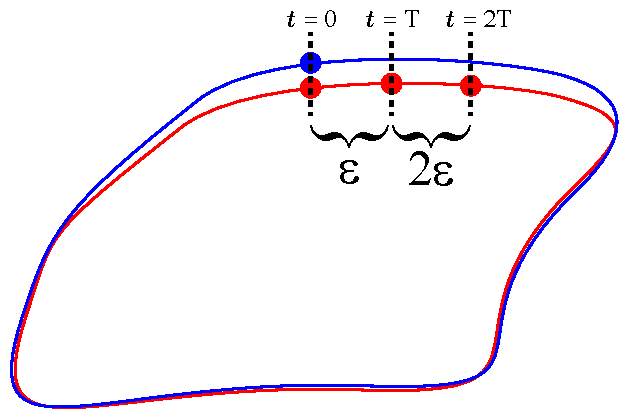
\includegraphics[width=0.5\textwidth]{lc_period_div}
  \caption{Divergence of orbits at limit cycles after $T$.
  Even though an approximation (red) might have an orbit that stays $\epsilon$ close to a target system with a stable limit cycle with period $T$ (blue), if the periods are not exactly matched, the two systems will diverge from each other.
  In this example, the approximation has period $\hat{T} = T+\epsilon$ and will hence be above the approximation guarantee at time $t=2T$.
  }\label{fig:lc_period_div}
\end{SCfigure}

Another example of divergence after $T$ arises around separatrices.
Points near a separatrix will converge to different attractors if there is a non-perfect match of separatrices (see Fig.~\ref{fig:separatrices}).
We will refer to this as \textbf{B-type error} (for \textbf{B}asin).



%FPS%fading%FMS%FMP
\subsubsection{Approximation of fading memory systems}\label{sec:fadingmemory}
%On the general theory of fading memory \citep{coleman1968general}
The concept of a system having the fading memory property (FMP) has been a cornerstone in the study of dynamical systems\citep{coleman1968general}, providing a framework where the system’s output depends on past inputs with gradually diminishing influence \citep{boyd1985fading}.
That the output of a dynamical relationship should depend only on the recent past of its input and that the effect of the distant past should fade away is intuitively clear  \citep{sepulchre2021fading}.
%-APPROXIMATION BY VOLTERRA SERIES: A simplified interpretation of the N -th Volterra Series expansion is the “N -th Taylor expansion in the sequence variable x”.
%-APPROXIMATION BY FINITE-DIMENSIONAL DYNAMICAL SYSTEMS

Here, we will present some UAP results where target systems have some FM-like property.
However, while these results are promising, they are limited in scope.
The requirement of fading memory inherently restricts the class of dynamical systems that can be effectively approximated.
Many real-world systems exhibit behaviors where the influence of past inputs does not simply fade away over time; instead, they can have long-term dependencies or even cyclical behaviors that are crucial to their dynamics.
A very simple example is a system with two stable fixed points.
We now discuss existing universal approximation results that are confined to fading memory systems and critically assess their limitations.



\begin{definition}[Fading memory Property (FMP)]
Let $x_1, x_2$ be bounded sequences indexed by $\mathbb{R}$, and let $H$ be a sequence of causal, shift-equivariant (also called time-homogeneous) functionals.
Here, causal means $H_t(x) = H_t(x(-\infty,t])$ for all $t$.
We say that $H$ has the \textbf{FMP} if there is a monotonically decreasing function $w : \mathbb{R}^+ \to (0, 1]$ such that for any $\varepsilon > 0$ there exists $\delta > 0$ with 
\[
|H_t(x_1) - H_t(x_2)| < \varepsilon \quad \text{whenever} \quad \sup_{s \in (-\infty, t]} |x_1(s) - x_2(s)| w(t - s) < \delta.
\]
\end{definition}
%The notion of fading memory is strictly an input/output property, that is, it refers only to the operator $\mathcal{H}$ which maps inputs into outputs; the realization of $\mathcal{H}$ (there need not even be one) is irrelevant.

Typically, the FMP is used to reduce the approximation problem to one over a finite, bounded index set, and then appeal to the density of fully connected neural network to obtain approximation \citep{gonon2021fading}. %more examples


\paragraph{Linear RNNs}
\citet{li2020curse} and \citet{li2022approximation} investigate Linear RNNs in continuous time, % and therefore linear functionals
proving that linear RNNs can approximate continuous, linear, causal, regular and time-homogeneous functionals. % on $\mathcal{X}$ .
Of course, regular linear functionals have fading memory: their dynamics converge to zero at infinite time ($\lim_{n\rightarrow\infty} H(x(n)) = 0$) and therefore such results are trivial.
 

\paragraph{Exponential decaying memory}
State Space Models (SSMs) with layer-wise nonlinearity are universal approximators of systems with exponential decaying memory \citep{wang2024state}.


\paragraph{Uniform asymptotic incremental stability}
Uniform asymptotic incremental stability was introduced in \citep{pavlov2006uniform}.
UAP of RNNs for uniformly asymptotically incrementally stable systems on an infinite time horizon\citep{hanson2020universal, hanson2021learning}.


\paragraph{Reservoir computing}
%\paragraph{ESN}
\citet{jaeger2001echo} proposed Echo State Networks (ESNs), demonstrating their universal approximation capabilities specifically for fading memory systems.
This result was extended to include approximation of systems with an input \citep{manjunath2013echo}.
%ESNs are universal uniform approximators  for discrete-time fading memory filters with uniformly bounded inputs \citep{grigoryeva2018echo,grigoryeva2018universal}. 

For neuroscience \citep{auslender2024decoding}

If the domain of the functional $H$ is restricted to a space of uniformly bounded sequences with the fading memory property then various families of state-space transformations can be used to approximate it uniformly: 
 linear systems with polynomial or neural network readouts \citep{boyd1985fading,grigoryeva2018universal,gonon2019reservoir}, state-affine systems with linear readouts \citep{grigoryeva2018universal}, or echo state networks \citep{grigoryeva2018echo,gonon2019reservoir,gonon2021fading,gonon2023approximation}.
 More recently, Simple Cycle Reservoirs were shown to be universal for this set of systems \citep{li2023simple}.
% In other words, any of these families exhibit universality properties in the fading memory category.
Finally, a new method was developed to approximate Fading Memory Systems (FMS) by using a kernel representation (instead of a state-space representation) of the model \citep{huo2024kernel}. %approximate all fading memory functionals

%Echo state networks are universal \citep{grigoryeva2018echo} [Grig 18a]
%Universal discrete-time reservoir computers with stochastic inputs and linear readouts using non-homogeneous state-affine systems \citep{grigoryeva2018universal} [Grig 18b]
%Risk bounds for reservoir computing \citep{gonon2020risk} [Gono 20a]
%Reservoir computing universality with stochastic inputs \citep{gonon2019reservoir} [Gono 20b]
%Fading memory echo state networks are universal \citep{gonon2021fading} [Gono 21]
%Approximation error estimates for random neural networks and reservoir systems \citep{gonon2023approximation} [Gono 23a]

%Universal Transformer
 \citet{dehghani2018universal} introduce a recurrently-stacked universal transformer and demonstrate its effectiveness on text understanding and generation and subsequently, transformer models are universal approximators of continuous permutation equivariant sequence-to-sequence functions with compact support \citep{yun2019transformers}.


% Deep Equilibrium Sequence Model (encapsulates universal transformer) and are themselves an instance of the so-called implicit-depth models such as neural ordinary differential equations
Recently, \citet{bai2019deq} proposed the deep equilibrium model (DEQ) which is equivalent to running an infinite depth (weight-tied) feedforward network and which was shown to be able to approximate any sequence whose underlying dynamics is determined by a model that converge to a fixed point.
This model was further extended to be able to capture systems with arbitrary invariant sets, but the UAP has not been established \citep{konishi2023stable}. %some remarks: p.397


\subsubsection{FMP makes approximation results trivial} %put in prev section?
 The input forgetting property (also referred to in the literature as the unique steady-state property) is a modeling feature that appears profusely in applications and that can be obtained out of the so-called fading memory property.
In fact, every fading-memory system could be uniformly approximated arbitrarily closely over the set of systems with 'linear dynamics'\citep{matthews1993approximating}. %Theorem 3+4
Using the perceptron to uniformly approximate the external representation of a fading-memory system results in a finite-memory system model, called the perceptron filter \citep{matthews1993approximating}.
%
If  input/output sequence target has a realization\footnote{See Supp.Sec.~\ref{sec:realization}.} as a dynamical system, then the fading memory property is related to the unique steady-state property for dynamical systems \citep{chua1976qualitative}.
Hence, the fading memory assumption implies that the state will be “asymptotically independent” of the initial condition.
Therefore, FPM systems cannot have multi-stability which makes this framework exclude many real-world systems.

 
\begin{remark}
The FMP quantitatively captures the idea that perturbations to the initial condition have asymptotically negligible influence on the long-term behavior of the system trajectory.
This implies that imperfect system models may still be able of generating outputs that uniformly approximate the outputs of the original system over infinite time intervals.
In contrast, for systems not satisfying this stability condition, a sharp bound on the approximation error degrades exponentially with time \citep{hirsch1974nonautonomous, sontag2013mathematical}.
\end{remark}

%Stability and memory-loss go hand-in-hand \citep{manjunath2020stability}


Why should we assume that the underlying dynamics in neural networks converge to a fixed point?
Models of neural computation should cover a broader class of dynamics, e.g, oscillations \citep{townley2000existence, kag2020rnns, chang2019antisymmetricrnn,rapp1987periodic}. %could convey preferred capabilities in learning 




%\paragraph{Stability implies FNNs are enough}%crit
%When Recurrent Models Don't Need to Be Recurrent \citep{miller2018stable}.





%%%%%%%%%%%%%%%%%%%
\paragraph{Topological equivalency}
ESNs can be trained to have  topologically conjugate dynamics to structurally stable dynamical systems \citep{hart2020embedding}.
This does guarantee knowledge of the dynamics beyond a finite time horizon.
However, this is trivial for approximation of structurally stable systems with NODEs.
It is true by virtue of Theorem.~\ref{theorem:ss} that vector fields that are close to the vector field of a dynamical system will have dynamics that are topologically conjugate to it.
Because it is well known that vector fields can be approximated to arbitrary precision with FNN, this result immediately follows for NODEs.

%the autonomous ESN ψ ∈ C 1(Rd) with parameters ( A,  W in, W out,  φ) has a normally hyperbolic attracting submanifold on which ψ is topologically conjugate to φ.

Fixed point and limit cycle matching \citep{cohen1992construction}.


\section{Approximation of multi-stable dynamical systems on infinite time intervals}
\paragraph{Roadmap}
First we describe the target (the systems we can approximate) and hypothesis classes (the systems that we approximate with) and the metric for the density result (way we measure how wrong our approximation is to our target system).
Then, we prove our universal approximation property for this setting by step-wise constructing the target class:
starting with autonomous systems with a finite number of hyperbolic fixed points,
then systems with (additionally) a finite number of hyperbolic limit cycles
and finally, covering approximation of chaotic orbits.
We then extend these results to non-autonomous dynamical systems.



\subsection{The problem of approximation}\label{sec:approximationtheory} %{Problem statement}
For behaving agents we can formalize their behavior as sequence-to-sequence or input-output mappings.
We will call $\mathcal{X}$ the space of input sequences and $\mathcal{Y}$ the space of output sequences.

We consider a family of target functions, or simply targets, which is a subset \(\mathcal{C} \) of all mappings \( \mathcal{X} \rightarrow \mathcal{Y} \), i.e., \( \mathcal{C} \subset \mathcal{Y}^\mathcal{X} \). 
These are the relationships we wish to approximate (or ``learn"), by some (simpler or at least parameterized) candidate functions.
Let us denote this set of \textbf{candidates} by \( \mathcal{H} \subset \mathcal{Y}^\mathcal{X} \).
In learning theory, this is often called a \textbf{hypothesis space}.
The problem of approximation concerns how well functions in \( \mathcal{H} \) can resolve functions in \( \mathcal{C} \).
This is typically formulated in terms of a bound on the (maximal) error between the approximation and the target mapping.

We will discuss what the space is of target dynamical systems that we can approximate.
Furthermore, these can be approximated in a particular way, i.e. with a specific difference between the approximant and the target system (the metric).
This difference is measured as the expectation of the uniform norm difference between the flows. 
We can make the probability of finding a trajectory of the approximation to be off by a certain arbitrary threshold arbitrarily small. 


We start by showing the UAP for our hypothesis class (see Sec.~\ref{sec:hypothesis}) for structurally stable systems with a finite set of fixed points.
Then we extend this results where we consider systems with a finite set of periodic orbits.
We then also include systems that additionally have a finite set of continuous attractors.
We conclude with how these results extend to a class of non-autonomous dynamical systems and some remarks about approximation of chaotic orbits.
Each of these results considers approximation of a system on a compact space that is globally attractive. %explain what this entails



\subsubsection{Target class}\label{sec:target}
%Autonomous
%Structurally stable+Fixed points = hyperbolic fixed points
%The dynamics is globally attractive / There exist a compact set that with the fixed points inside that is forward invariant 
For our approximation results, we consider the following dynamics:
\begin{equation}
\dot x = f(x)   \ \ \ f\in C^1.
\end{equation}


\subsubsection{Hypothesis class}\label{sec:hypothesis}
%rename f hat?
The hypothesis class $\mathcal{G}$ is composed of
\begin{equation}
\dot x = g(x) 
\end{equation}
where $g$ is an FNN with the universal approximation property.
In essence, by setting up $g$ as a neural network, you are equipping the NODE with a highly flexible model for $g$, which can approximate a vast variety of continuous functions. 

These restrictions of the hypothesis class are Bernstein-type results (in the classification of approximation result types made in \citep{jiang2023brief}).
%analogy with realization of transfer functions in state space models


\subsubsection{Metric}\label{sec:metric}
First, of all, we compare trajectories through the uniform norm over time (given the same initial starting point \citep{girard2007approximation}):
\begin{equation}
\|\varphi(t,x_0)-\hat \varphi(t,x_0)\|_\infty = \sup_t|\varphi(t,x_0)-\hat \varphi(t,x_0)|.
\end{equation}

We consider a compact $X$ on which we measure the difference between the target and our approximation.
\footnote{FNN approximation universality is also on compact intervals.
The results can be extended to systems that diverge to infinite in a finite number of orbits (all orbits that diverge converge in uniform norm to one of these divergent orbits).}
%
Expectation of the error over all initial points (similar to the metric in \citep{hammer2000approximation} and \citep{hanson2021learning}):
\begin{equation}
%\|\varphi-\hat \varphi\|_\epsilon \coloneqq \frac{1}{\vol X}\mathbb{E}\left[ \int_{x_0\in X}   \mathds{1}[\|\varphi(t,x_0)-\hat \varphi(t,x_0)\|_\infty>\epsilon]\right],
\|\varphi-\hat \varphi\|_\epsilon \coloneqq  \mathbb{P}\left(\|\varphi(\cdot,x_0)-\hat \varphi(\cdot,x_0)\|_\infty>\epsilon\right).
\end{equation}
%where $\mathds{1}[\cdot]$ is the indicator function. 


%why we cannot stricten the metric
For a multistable system it is not possible to find a universal approximation result if we consider a more strict notion of difference between the target and approximant.
For example, if we take the uniform norm of the uniform norm, it can be shown that there is always a system with a separatrix that can not be exactly matched which would lead to an error that is the distance between the two $\omega$-limit sets.

%\subsubsection{Guarantee in $N\rightarrow\infty$ or at finite $N$}
%It could be that existing theorems could be interpreted that in the limit $N\rightarrow\infty$ the approximation holds. %e.g.\citep{podlaski2024approximating}
%ie $\lim_{N\rightarrow\infty} error = 0$
%Here we do it for finite $N$.
%ie for each $\epsilon>0$ $\exists N$ such that $error(N) < \epsilon$
%(implies the above limit)




\subsection{Approximating systems with a finite number of hyperbolic stable fixed points}
\begin{theorem}
Let $D$ be an open subset of $\mathbb{R}^n$,
 $f\colon D \to \mathbb{R}^m$ be a $C^1$-mapping,
  and $I$ be a compact subset of $D$ such that any solution $x(t)$ with initial value $x(0) \in I$ of an ordinary differential equation
\begin{equation}\label{eq:5}
    \dot{x} = f(x), \quad x(0) \in D
\end{equation}
is defined for $t\in\reals_{+}$ and $x(t)$ is included in $I$.
This defines a flow $\varphi(\cdot, \cdot)$.


Then, for an arbitrary $\epsilon, \delta > 0$, there exist an MLP recurrent neural network 
 \begin{equation}
\dot x = \hat f(x) = \sigma(A\sigma(Bx+b)+a)
\end{equation}
%such that for a solution $\hat \varphi(t,x_0)$ satisfying Eq~\ref{eq:5} with initial state $x_0$ of the network
such that its flow $\hat \varphi$ satisfies
\begin{equation}
\|\varphi-\hat \varphi\|_\epsilon < \delta.
\end{equation}
\end{theorem}

%proof will be at end of section? 
%establish necessary pieces as propositions

\begin{proposition}
The fixed points and limit cycles of $C^1$ ODEs can be arbitrarily closely approximated in the $\|\varphi-\hat \varphi\|_\epsilon < \delta$ flow sense.
\end{proposition}

\begin{proof}
%%%top eq
Because of the density of the hypothesis class $\mathcal{G}$ we have that for any $f\in C^1$ and any $\epsilon>0$
there exists $\hat f\in\mathcal{G}$ such that $\|f-\hat f\|<\epsilon$.
%
Structural stability implies that there exists a $\delta>0$ such that for all $g\in C^1$ that are $\delta$ $C^1$ close to $f$, the flow is topologically equivalent to that of $f$.
%
So we can choose $\delta$ such that for all $\|f-\hat f\|<\delta$ the flow of $\hat f$ is topologically equivalent to that of $f$.

ADD: fixed points of $\hat f$ are $\mathcal{O}(\epsilon)$ close to $f$.
\end{proof}

This establishes that for all $\epsilon>0$ there is some time $T$ for which for all $t>T$ we have that $x(t)-\hat x(t)<\epsilon$.


\paragraph{A tale of two errors}
Note that the above error bound depends on two separate quantities: the local error 
$\| f(s; \tilde{\varphi}_0, s(x)) - f(s; \tilde{\varphi}_0, s(x)) \|$ 
 and the term 
$\| D\varphi_{s,t}(\tilde{\varphi}_0, s(x)) \|$, 
which bounds the sensitivity of the flow $\varphi_{s,t}(x)$ to an infinitesimal perturbation of its initial condition.
%TODO: more catchy name for type I error: F-type (Flow)
We can bound these two types of errors as follows.%error^I and error^II


\setlength\belowcaptionskip{-1ex}
\begin{SCfigure}[10][bthp]
  \centering
  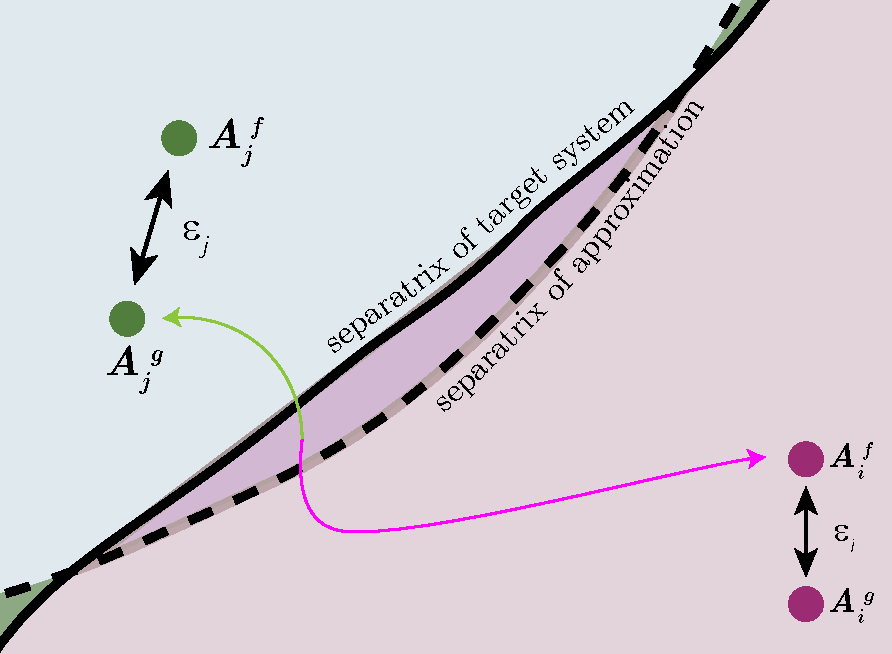
\includegraphics[width=0.5\textwidth]{separatrices}
  \caption{
	A mismatching pair of separatrices between attractors $A_i$ and $A_j$.
	The target subsystem has two stable fixed points ($A_i^f$ and $A_j^f$) with separation between the basins of attraction by the separatrix (black line).
	The approximation also has two stable fixed points ($A_i^g$ and $A_j^g$ at slightly different locations) but with a separatrix that is close to the target one but is not perfectly on it (dashed line).
	All the points in the red region go to $A_i^f$ for the target system and to $A_i^g$ (that is at an $\epsilon_i$ distance) for the approximation. Similarly for the other stable fixed point for initial points in the blue region.
	This target system will have a set of points (in the green region) that if the flow is initialized there it has $A_i^f$ as the $\omega$-limit set (magenta line), however for the approximation the flow will approach $A_i^g$ (green line).
	The opposite mismatch is true for the purple region.
	%(such a model can be found in e.g. \citep{wong2007evidence})
  }\label{fig:separatrices}
\end{SCfigure}

\subsubsection{Errors inside an intersection of the Basins of Attraction (BoA) of the target and approximation}
So if we have $x_0\in BOA(A_i^f) \cap BOA(A_i^g)$, the flow deviates along the trajectories up to 
\[
\|\varphi_{0,t}(x) - \tilde{\varphi}_{0,t}(x)\| \leq \int_0^t \|D\varphi_{s,t}(\tilde{\varphi}_{0,s}(x))\| \|f(s; \tilde{\varphi}_{0,s}(x)) - g(s; \tilde{\varphi}_{0,s}(x))\| \, ds.
\]
Prop.~\ref{prop:313} from \citep{vanhandel2007filtering}, see Supp.Sec.~\ref{sec:313}.
%
See Rem.~\ref{rem:313}.

The first term \[\|D\varphi_{s,t}(\tilde{\varphi}_{0,s}(x))\|\]
is bounded. %?
Define $M\coloneqq \sup \|D\varphi_{s,t}(\tilde{\varphi}_{0,s}(x))\|<\infty$. 

Additionally:
\(\|D\varphi_{s,t}(\tilde{\varphi}_{0,s}(x))\|\rightarrow 0\) for \(t\rightarrow\infty\).
%
This guarantees that the integral is finite.

The second term
\[\|f(s; \tilde{\varphi}_{0,s}(x)) - g(s; \tilde{\varphi}_{0,s}(x))\|\]
can be made arbitrarily small because of the UAP for mappings.


TODO:
orbits from these initial conditions converge to $\omega$-limit sets that are at most $\epsilon_i$ Hausdorff distance from each other.


This guarantees that the integral can be made arbitrarily small.	
%conclusion about Type I errors
Hence, there exists an FNN that defines a vector field for which for each attractor we have $\epsilon_i<\epsilon$. 



%Consider separately ?
%1 orbits to fixed points: path starting at $x_0$ is finite
%2 orbits to stable limit cycles.



%TODO: more catchy name for type II error: B-type (Basin) 
\subsubsection{Errors at the boundary of a BoA}%type II
The other type of error arises because trajectories go to different attractors, i.e., $x_0\in BOA(A_i^f,A_j^g)$ for $i\neq j$.
For such initial points the error along the flow cannot be bounded.
Eliminating this type of error would constitute perfectly matching the separatrices which can not be guaranteed.
We can reduce the volume in of initial points for which this type of error arises, by reducing the mismatch between the separatrices (proportional to the distance between the attractors).

The volume for which type II error arises is 
\[\sum\boa(A_i^f)\cap\boa(A_i^g).\]



\paragraph{Boundary of BoA is persistent}
The boundary of the BoA of attractor $A_i^f$ is %BoAs are open sets
\[\partial\boa(A_i) = \overline{\boa(A_i^f)} \cap (X - \overline{\boa(A_i^f)}).\]
where \(\overline{\cdot}\) denotes the closure of a set. Same as \(\cl\).
% =\cl\boa(A_i^f)-\boa(A_i^f)\.\]%this should hold for an open set...

Then for some value $\epsilon_{\operatorname{sep}}$ we have that 
\begin{equation}\label{eq:separatrixoverlap}
\bigcup_i \boa(A_i^f)\cap\boa(A_i^g) \subset \bigcup_i B_{\epsilon_{\operatorname{sep}}}(\partial\boa(A_i^f)). 
\end{equation}

The right hand side's volume is at most $\mathcal{O}(\delta)$ with $\leq\epsilon_{\operatorname{sep}}$ the Hausdorff distance between the total separatrix submanifolds.
This $\delta$ can be made arbitrarily low because of the FNN universal approximation results.

For each attractor $A_i$ we have that the boundary of the basin of attraction $\partial(\boa(A_i^f))$ is a compact normally hyperbolic invariant manifold (See Supp.Sec.~\ref{sec:boaboundary}).
Consider the connected components $B^f_{ij}$ of $\partial(\boa(A_i^f))$.
%\footnote{For example,  all invariant manifolds of ReLU RNNs are either continuous attractors (in the direction of non-normal hyperbolicity) or normally hyperbolic.}
Then, by Fenichel's Persistent manifold theorem, there exists a $\delta_{ij}$ such that for all $g$ that are $\delta_{ij}$ $C^1$ close to $f$ such that $g$ has a normally hyperbolic invariant manifold  $B^g_{ij}$ that is diffeomorphic to and at most at $\mathcal{\delta_{ij}}$ Hausdorff distance from $B^f_{ij}$.
Therefore, by Eq.~\ref{eq:separatrixoverlap}, the overlap of the separatrices is less than $\mathcal{O}\epsilon_{\operatorname{sep}}$.%TODO: figure out bound on the volume
%compactness should imply that the volume is at most $\mathcal{\epsilon_{\operatorname{sep}}$.
Therefore, there is $k_{ij}\in\reals$ such that the Hausdorff distance between $B^f_{ij}$ and $B^g_{ij}$ is $k_{ij}\delta_{ij}$.
Let  $N_{\operatorname{cc}}$ be the number of connected components of $\partial(\boa(A_i^f))$.
Choose $\delta_{ij}<k_{ij}\delta/N_{\operatorname{cc}}$.%the global \delta....
Define $\delta_i\coloneqq\sum_{i=1}{N_{\operatorname{cc}}}\delta_{ij}$.

%simplifying:%we can consider $\cl\boa(A_i) to be an invariant manifold with boundary

%move to end of subsection:
Now we need to sum all the different errors together.
We get a bunch of $\delta_i$'s.
%Take $\epsilon_i<$.??
Then $\delta_i< \frac{\delta}{N_{\operatorname{attractors}}}$ for each $i$ and hence $\sum_i\delta_i<\delta$.


\paragraph{Alternative: isolating neighborhoods as persistent}
Isolating neighborhood with boundary that is transversal to flow.
The boundary can be taken to be arbitrarily close to the boundary of the BoA.
By taking the isolating neighborhood to be closer and closer to the BoA, we can prove persistence of separatrix.

%construction
Step 1: create inflowing isolated neighborhood.
%N-dim DS
Take $I$ to be a section in the tubular neighborhood of the fixed point.
 $\{\varphi(t,x_0) \mid x_0\in I\}$ forms a connected $N-1$ dimensional manifold for each $t$.
%2D DS: $\{\varphi(t,x_0) \mid x_0\in S^1\}$ forms a connected $1$ dimensional manifold for each $t$.
%1: More generally, take a section in the tubular neighborhood for $t=0$: $I_0 = \{\varphi(0,x_0) \mid x_0\in X_0\}$
The initial set of points is a connected manifold.
For each \( t \in \reals \), the image \( \{ \varphi(t, s) \mid s \in I \} \) remains a connected $N-1$ dimensional manifold because:

\begin{enumerate}
    \item The initial family \( \gamma(I) \) is a $N-1$ dimensional manifold.
    \item The map \( \phi(t, \cdot) \) is \( C^1 \) and thus an immersion.
    \item The image of a connected set under a continuous map remains connected.
\end{enumerate}
This forms the boundary of the isolating neighborhood.

%1.2: For limit cycles this is a torus-shaped 2D manifold (in 3D, in 2D it is union of 2 $S^1$s): relevant for next section.


For each $t\in\reals$ the set $I_t = \{\varphi(t,x_0) \mid x_0 \in X_0 \}$ is a manifold.
%
For each $t\in\reals$ the set $\bigcup_{s<t}I_s$ is an isolating neighborhood.


2: Let $t\rightarrow\infty$, then this isolating neighborhood fills up the basin of attraction

3: These manifolds are forward invariant for each $t$

4: Isolating neighborhoods of target and approximation have same Conley index (trivial) for each $t$ (if vector fields are close to each other, see Sec.\ref{sec:cit})

5: Separatrix must be in remaining part of the state space and, hence it is persistent (i.e., it is $\mathcal{O}(\epsilon)$ close)


%\subsubsection{Alternative: stable and unstable manifolds as persistent}
%stable and unstable manifolds of a normally hyperbolic manifold persist under perturbation Theorem 2.3.6 in \citep{kuehn2015multipletimescale}.
%
%Laminations: The collection of global stable/unstable manifolds. The same for the local stable/unstable manifolds or the local unstable manifolds for the geodesic flow on a compact manifolds with nonzero Lyapunov exponents almost everywhere. 
%Persistence of laminations \citep{berger2010persistence}



\subsection{Approximation of stable limit cycles}
%TODO:  name for type III error: L-type (limit cycle) P-type (period)
As we have seen in Sec.~\ref{sec:beyondfinitetime}, any mismatch in periods in the period of stable limit cycles introduces an error.
We will get convergence onto a limit cycle that is close in Hausdorff distance to the target limit cycle. %$\omega$-limit set?
But, for an approximation of the vector field we will in general have a small discrepancy in the periods between the two limit cycles that will lead to a uniform norm difference between the flows that is the maximal distance between all pairs of points on the two limit cycles.
This would make our method fail!
In our metric, this error is of the size of the volume of the basin of attraction for the limit cycle.
Is it possible to perfectly match target limit cycle periods?
We will describe a recipe for systems with single and multiple limit cycles.


\subsubsection{A single stable limit cycle}
%However, we can correct this discrepancy.
We have a difference in period $T-\hat T = \epsilon_T$
with \[T\coloneqq\frac{1}{\int_{LC}\|f(x)\|dx} \text{ and } \hat T\coloneqq\frac{1}{\int_{\hat{LC}}\|\hat f(x)\|dx}.\]
%
We will apply a perturbation $\bar{f}$ to our approximations that is small enough for the persistence of the limit cycle ($\delta$ needs to be small enough) 
so that 
\[\int_{\tilde{LC}}\|\tilde{f}(x)\| dx = \frac{1}{T}. 	\]% for the integrated vector field along the limit cycle $\int_{LC}f(x)$.
The existence of such a perturbation (i.e. that indeed it will be \emph{small} enough) requires that the initial difference between the periods is small.
If the approximation vector field is close enough to the target vector field, then the periods will be guaranteed to be close (see for the precise statement and proof Supp.Sec.~\ref{sec:periodcloseness}).
The resulting total approximation is \[\tilde{f}=%\hat{f}+\hat{\hat{f}} = 
 \hat{f} + a(\epsilon_T)(\hat{f} + \hat{\epsilon}\bar{f}).\]


We can use the fact that the tubular neighborhood of diameter $\delta_T$ around the limit cycle (LC) is an (inflowing) normally hyperbolic invariant manifold.
This implies that there is a 3 layer FNN that approximates the vector field x a bump function around the LC (similar idea as in paper but this would be an actual possible implementation).
Then we know that the this NHIM will persist.
We also know that there is a maximal perturbation size ($\epsilon_{LC}$) for which the limit cycle persists.
So we have to guarantee that the limit cycle approximation is already close enough so that this perturbation does not destroy the limit cycle.
We can now rescale the perturbation so that the period of approximation limit cycle matches the target's. 
We just increase or decrease  the above perturbation by multiplying with a scalar so that this equality holds.
The only thing we now need to worry about is how the length of the limit cycle changes as a result of this perturbation and whether we can indeed get the equality.

Fenichel's PMT guarantees that the perturbed limit cycle lies within $\mathcal{O}(\epsilon)$ the original limit cycle approximation.

%So if it gets longer because of the perturbation (i.e. $\hat \ell(\epsilon)$ is an increasing function) as long as $1/(\hat \ell+g(\epsilon))$ is not decreasing at the same rate there should exist a value $\epsilon$ for which the equality holds

%the fixed point happens at an epsilon that is small enough for the persistence of the other parts: TODO

%choosing the size of the tubular neighbourhood

\textbf{Knobs}
\begin{itemize}
\item $\epsilon_T$: small enough so that limit cycle is structurally stable
\item $\hat\epsilon$: needs to be small enough so that effect of correction outside of the tubular neighbourhood doesn't affect attractors and separatrices
\item $\delta_T$: needs to be small enough so that no other attractor or separatrix is included (will this have an effect on the inside-basin flow error?)
\end{itemize}

this implies that if $\delta T$ is small enough then $\epsilon_T$ is small

\paragraph{The effect of the correction on the flow inside the basins}
- Tubular neighbourhood: $\epsilon_T$ effect
- Outside $\hat\epsilon$ effect


\paragraph{The effect of the correction on the separatrices}
See note on  $\hat\epsilon$ Knob.


\paragraph{The basin of attraction for a stable limit cycle}
Regions of attraction to periodic orbits have an interesting structure: they must be a continuous deformation of a torus: the Cartesian product of an open unit disc of dimension $n-1$, with a scalar circle coordinate \citep{wilson1967structure}.



\paragraph{Summary}
We can choose the initial approximation $\hat{f}$ such that the period difference is smaller than $\epsilon_T$.
We can then choose a correction to the vector field in a tubular neighborhood around the limit cycle such that this difference is reduced to zero.


%%%%%%%%%%%%%%%%
\subsubsection{Multiple limit cycles}
We can perform the same procedure for a finite set of limit cycles.
We have to make sure that all the $\hat{\epsilon}_i$ are step-wise small enough so that $\epsilon_{T_i}$ is small enough. 

\[ \tilde f_i = (1+ \epsilon_{T_i})\hat{f}_i + \epsilon_{T_i}\hat{\epsilon}_i\bar{f}_i + \sum_{j\neq i}\epsilon_{T_j}\hat{\epsilon}_j\bar{f}_j\]

%can we really do this sequentially? no, we have to do it in parallel
%when we change a_T_i we have to adjust the other a_T_j s

 ReLU networks which can be made to be zero outside of the tubular neighbourhood as a method to make things work for multiple stable limit cycles?


%%%QPTA
\paragraph{Quasi-periodic toroidal attractors (QPTA)}%more generally: doing this for multiple limit cycles
Important!\citep{Park2023a}



%%%%%%%%%%%%%%%%
%%%CA
\subsection{Approximating a continuous attractors}\label{sec:chaos}
%TODO:  name for type V error: D-type (discretization) 
%for the extension of continuous attractors we need to assume that all maximally invariant sets are normally hyperbolic

%continuous attractor (zero flow)
We can tile the continuous attractor with a uniform grid of stable fixed points.
Each of the neighbouring stable fixed points can be at most $\epsilon$ apart.
This is structurally stable dynamics, so we can approximate its vector field with $\epsilon$ accuracy and we are guaranteed to have a topologically equivalent system to it with the fixed points being moved at most $\mathcal{O}(\epsilon)$.

See \citep{Sagodi2024a}.


%continuum of attractors (nonzero flow): e.g. torus
We can tile the continuous attractor with a uniform grid of stable limit cycles.


%\subsection{Center manifolds}
%???



%%%%%%%%%%%%%%%%%%%%%
\subsection{Approximating a chaotic orbit}
%TODO:  name for type IV error: C-type (chaos)
We cannot approximate according to our above criteria.
Every small discrepancy in the vector field will lead to orbits starting at same position to diverge over time, analogous to perturbing initial start of the chaotic orbit.


What we can do is minimize the Hausdorff distance between the chaotic invariant manifolds and match the Lyapunov exponents of the target system
The first because of structural stability.
%%The second because of ???


Alternatively, we can guarantee that the shift representation of the dynamics is persistent.
% Symbolic dynamics: Mapping onto the same shift dynamical system

\paragraph{Why?} 
Forecasting
\citep{jaeger2004harnessing}
\citep{fan2020long}
\citep{vlachas2020backpropagation}
\citep{grigoryeva2024forecasting}

\paragraph{How?}
Attractor reconstruction, reconstructing the full Lyapunov spectrum of a dynamical system using reservoir computing \citep{hart2024attractor}

Different metric: Chaotic orbits
mention: we can guarantee finite time approximation
prove: we can never do infinite time approximation 



\section{Input-driven dynamics}

This can be only done by also calculating in the probability of making an error on a given input.
So the approximation probability guarantee will need to be formulated in terms of the probability of making an error bigger than a threshold calculated over the function of input sequences and initial points.

For non-autonomous we need another Bernstein-type result:
we can only approximate input driven dynamics (in our metric) if a forward attractor exists for each input sequence 
This allows us to formulate approximation in terms of attractors and separatrices (but now in input space)

If an input sequence doesn't converge (i.e. it has a mixing property) we get the same issue with approximating the system as with chaotic orbits.



\subsection{Asymptotically autonomous dynamics}


\subsection{Contractive dynamics}

\begin{theorem}[Theorem 2 in \citep{lohmiller1998contraction}]\label{thrm:contractive}
Given the system equations $\dot x = f(x,t)$, any trajectory, which starts in a ball of constant radius with respect to the metric $M(x,t)$, centered at a given trajectory and contained at all times in a contraction region with respect to $M(x,t)$,  remains in that ball and converges exponentially to this trajectory.
\end{theorem}

\begin{remark}
Theorem \ref{thrm:contractive} actually corresponds to a necessary and sufficient condition for exponential convergence of a system. In this sense it generalizes and simplifies a number of previous results in dynamic systems theory.
\end{remark}

\begin{remark}
A convex contraction region contains at most one equilibrium point, since any length between two trajectories is shrinking exponentially in that region.
\end{remark}


\subsubsection{Limit cycles and contractivity}
\citep{manchester2014transverse} and refs therein: e.g. 16-20



\subsection{Finite-time horizon approximation + asymptotically autonomous = Infinite-time horizon approximation}









\section{Discussion}
\paragraph{Recap}	


\paragraph{Limit cycles}
Stable limit cycles are approximable but their approximation is not robust! (period will change under almost all perturbations)


\paragraph{Link to Total integrated error (TIE)}
We can look at the total integrated error between the target and the approximant and derive a similar UAP theorem.

Error is then defined as 
\begin{equation}
\operatorname{TIE}(\varphi, \hat{\varphi}) = \int_{x_0\in X}\|\varphi(t,x_0) - \hat{\varphi}(t, x_0)\|_\infty.
\end{equation}

It is then easy to show that $\forall\epsilon>0$ there exists a NODE such that $\operatorname{TIE}(\varphi, \hat{\varphi})<\epsilon$.

\paragraph{Link to MSE loss}
In the limit that $\delta\rightarrow 0$ and $\epsilon\rightarrow 0$  we have that 
\[\operatorname{MSE}(\varphi, \hat{\varphi}) \coloneqq \int_{x_0\in X} \|\varphi_t(x_0) - \hat{\varphi}_t(x_0)\|_\infty \rightarrow 0.\]


Limit $\delta\rightarrow 0$: error of type II goes to zero, i.e., perfectly matching separatrices


Limit $\epsilon\rightarrow 0$: error of type I goes to zero (apart from small mismatch around separatrices), i.e., perfectly matching in-basin dynamics


\paragraph{NODEs vs RNNs}
NODEs Simulate RNNs 
- Each NODE is state space equivalent to an RNN that is split into a part for which the equivalence holds and a hidden part (Boltzmann Machine-like)
-Each RNN is state space equivalent to an RNN



NNs as controllers \citep{sontag1992neural}


\paragraph{The price of universality}
This construction is immensely inefficient

Better to just look at RNNs. 


%%%%
\subsection{Implications for understanding neural computation} 

Reconstructing Computational Dynamics from Neural Measurements with Recurrent Neural Networks \citep{durstewitz2023reconstructing}.

Use of NODEs in neuroscience \citep{kim2021inferring}.


\paragraph{Models that generalize over time}


\paragraph{Interpretability}%move to anti-truncated koopman operator paper?

%\subsection{Convergent realism}

\paragraph{Robust neural computation}
Idea: Two dynamical phenomena are isolated into primitive architectural components which perform the operations of continuous nonlinear transformation and autoassociative recall \citep{pineda1988dynamics}.




\newpage
\bibliography{../all_ref.bib,../catniplab.bib}



\newpage
\appendix 

\section{Universal Approximation with Feedforward Neural Networks (FNNs)}\label{sec:uniapproxffn}

The foundation of our approach lies in leveraging the \textit{universal approximation property} of feedforward neural networks (FNNs) \citep{poggio1990networks}, a powerful result that makes neural networks exceptional for a broad array of tasks. This property allows FNNs to approximate complex functions with remarkable flexibility, providing the theoretical basis for their widespread success in machine learning.
For an overview see \citep{blum1991approximation,scarselli1998universal,augustine2024survey}.





\subsection{The Universal Approximation Theorem}
The universal approximation theorem states that a \textit{feedforward neural network} with at least one hidden layer, using a non-linear activation function (such as the sigmoid or ReLU), and equipped with enough neurons, can approximate \textit{any continuous function} defined on a compact subset of \(\mathbb{R}^n\) to arbitrary precision.

Formally, for any continuous function \(f(x)\) and any \(\epsilon > 0\), there exists an FNN such that:
\[
| f(x) - f_{\text{MLP}}(x) | < \epsilon \quad \forall x \in K
\]
where \(K \subset \mathbb{R}^n\) is compact. This guarantees that given sufficient resources (neurons, depth), the FNN can approximate \(f(x)\) as closely as desired within this bounded region.

The importance of the compact domain assumption is that it constrains the input space to a finite region, ensuring the approximation remains well-behaved.	
This is where the theorem’s beauty shines: while we often don’t know the explicit form of the target function, neural networks learn it purely from data, making them excellent for tasks like regression, classification, and pattern recognition.

 For example, sums of polynomial functions are known to have this property\citep{llavona1986approximation}

\subsection{Activation functions} %Sigmoidal 
At the heart of the theorem lies the activation function. Any non-linear, continuous, and non-constant function enables the network to approximate continuous functions universally.
A classic example is the \textit{sigmoidal function}, defined by the property:
\[
\lim_{x \to -\infty} \sigma(x) = 0 \quad \text{and} \quad \lim_{x \to +\infty} \sigma(x) = 1
\]
Many popular activation functions, such as the logistic sigmoid and tanh, fall into this category.
These functions introduce the necessary non-linearity, enabling the network to break free from the constraints of purely linear transformations.

%non-sigmoidal activations like the \textit{Rectified Linear Unit (ReLU)} 
Despite ReLU's unbounded nature, it still supports the universal approximation property, as shown in \citep{yarotsky2017error}.

\citep{mhaskar2019function}

\subsection{The Multi-layer Perceptron (MLP)}

The universal approximation property of FNNs was first proven by \citep{cybenko1989approximation} for sigmoidal activation functions. This was followed by significant generalizations by \citep{hornik1989multilayer}, \citep{funahashi1989approximate} and \citep{hechtnielsen1992backpropagation}, which extended the result to broader classes of activation functions, including the popular ReLU.
These results serve as the cornerstone of modern neural network theory, supporting the use of deep architectures across diverse machine learning applications.

% There is a single hidden layer feedforward network that approximates any measurable function to any desired degree of accuracy on some compact set K \citep{hornik1989multilayer}.

%all above are 3 layer FNNs? right?

Let’s now focus on the structure of a \textit{multi-layer perceptron (MLP)}, a common form of FNN. For a simple 3-layer MLP, the output can be expressed as:
\[
h^{(1)} = \sigma(W^{(1)} x + b^{(1)})
\]
\[
f_{\text{MLP}}(x) = W^{(2)} h^{(1)} + b^{(2)}
\]
Here, \(h^{(1)}\) represents the hidden layer, while \(W^{(1)}, W^{(2)}\) and \(b^{(1)}, b^{(2)}\) are the weights and biases learned during training. The activation function \(\sigma(\cdot)\) introduces the necessary non-linearity.


Three-layered multi-output Feedforward Networks are universal approximators for vector-valued functions \citep{irie1988capabilities}.

\begin{theorem}[Universal Approximation Theorem for Feedforward Neural Networks\citep{hornik1989multilayer,schafer2007uap}]
%\textbf{Theorem 1 (Universal Approximation Theorem for Feedforward Neural Networks).} 
For any sigmoid activation function \( f \), any dimension \( I \), and any probability measure \( \mu \) on \( (\mathbb{R}^I, \mathcal{B}^I) \), \( \Sigma_I(f) \) is uniformly dense on a compact domain in \( C^I \) and \( \rho_{\mu} \)-dense in \( M^I \).
\end{theorem}

\begin{corollary}%[in \citep{schafer2007uap}]
Theorem 1 holds for the approximation of functions in \( C^{I,N} \) and \( M^{I,N} \) by the extended function class \( \Sigma^{I,N} \). Thereby, the metric \( \rho_{\mu} \) is replaced by \( \rho_{\mu}^N := \sum_{k=1}^{N} \rho_{\mu}(f_k, g_k) \).
\end{corollary}

%In a more general case, for a deeper MLP with \(L\) layers, we have:
%\[
%h^{(1)} = \sigma(W^{(1)} x + b^{(1)})
%\]
%\[
%h^{(2)} = \sigma(W^{(2)} h^{(1)} + b^{(2)})
%\]
%\[
%\vdots
%\]
%\[
%h^{(L-1)} = \sigma(W^{(L-1)} h^{(L-2)} + b^{(L-1)})
%\]
%\[
%f(x) = W^{(L)} h^{(L-1)} + b^{(L)}
%\]

%This architecture allows the MLP to progressively build complex representations, layer by layer, transforming raw input data into rich feature hierarchies.%
%For the approximations, we either need to let the width or depth of the MLP grow.

It is not the specific choice of the activation function but rather the multilayer feed-forward architecture itself that gives neural networks the potential of being universal approximators\citep{hornik1991approximation}.
%
The universal approximation property is equivalent to having a nonpolynomial activation function \citep{pinkus1999approximation}.

\citep{mhaskar1997neural}
\citep{leshno1993multilayer}

UA with Deep narrow \citep{kidger2020universal}

with WTA networks \citep{maass2000wta}

Function+Derivatives \citep{hornik1990universal}
function and derivative \citep{li1996simultaneous}


\subsection{Other results on UAP for mappings}
NODEs are $L^p$-universal approximators \citep{li2022deep,li2022deeparxiv}
%invariant functions
\begin{remark}
The universal approximation property with respect to the $L^p$-norm can be insufficient as it does not guarantee an approximation for the entire input domain:
 $L^p$ approximation may still hold even if the approximator largely differs from the target function on a small region of the input space.
\end{remark}


Universal approximation of 
\begin{itemize}
\item Homeomorphisms \citep{zhang2020approximation}
\item Invariant functions\citep{li2022deep}
\item Monotone analytic functions homotopic to the identity\citep{tabuada2020universal}
\end{itemize}

\citep{tabuada2022universal}
\citep{marchi2021training}


\section{Neural ODEs (NODEs)}
%\subsection{}
Neural ODEs \citep{chen2018neural} represent the latest instance of continuous deep learning model for time series, first developed in the context of continuous recurrent networks \citep{cohen1983absolute}.
%
Neural ODEs model the continuous trajectory of the hidden state \( \mathbf{h}(t) \) as the solution to an ordinary differential equation parameterized by a neural network. Mathematically, the dynamics are defined by:

\[
\frac{d \mathbf{h}(t)}{dt} = f(\mathbf{h}(t), t, \theta)
\]

where \( \mathbf{h}(t) \) is the hidden state at time \( t \), \( f \) is a neural network with parameters \( \theta \), and \( t \) represents time. Given an initial condition \( \mathbf{h}(t_0) = \mathbf{h}_0 \), the evolution of the hidden state over time is computed by solving the ODE using numerical solvers, allowing the model to capture complex, continuous transformations.

%example of f
\textbf{Fully Connected Neural Network (Feedforward Network)}:

\[
f(\mathbf{h}(t), t, \theta) = W_2 \sigma(W_1 \mathbf{h}(t) + \mathbf{b}_1) + \mathbf{b}_2
\]

Here, \( \sigma \) is an activation function (e.g., ReLU, tanh, or sigmoid), \( W_1, W_2 \) are weight matrices, and \( \mathbf{b}_1, \mathbf{b}_2 \) are bias vectors.
 This form models the ODE dynamics using a simple two-layer feedforward network.

Universal approximation properties of neural operator architectures \citep{lu2021learning, kissas2022learning, kovachki2021universal}.


\paragraph{Applications}
%NODEs in neuroscience%
Neural ordinary differential equations (NODEs) are being increasingly adopted in computational and systems neuroscience, showing improved performance compared to current approaches \citep{kim2021inferring,geenjaar2023learning,sedler2023expressive,elgazzar2024universal,rubanova2019latent,coelho2024enhancing}.


%\paragraph{Latent}
%Latent ODE-RNN  \citep{rubanova2019latent}
%Latent ODE-LSTM \citep{coelho2024enhancing}

\paragraph{Time variant}
As continuous limits of ResNets, it is natural to take the coefficients of NODEs to be time-dependent.

semiautonomous NODEs (SA-NODEs) \citep{li2024universal}


\paragraph{Analysis}
\citep{massaroli2020nodes}




\section{Dynamical systems concepts}
\subsection{Fading memory}
\begin{definition}[Fading memory Property (FMP)]
Let $x_1, x_2$ be bounded sequences indexed by $\mathbb{R}$, and let $H$ be a sequence of causal, shift-equivariant (also called time-homogeneous) functionals.
Here, causal means $H_t(x) = H_t(x(-\infty,t])$ for all $t$.
We say that $H$ has the \textbf{FMP} if there is a monotonically decreasing function $w : \mathbb{R}^+ \to (0, 1]$ such that for any $\varepsilon > 0$ there exists $\delta > 0$ with 
\[
|H_t(x_1) - H_t(x_2)| < \varepsilon \quad \text{whenever} \quad \sup_{s \in (-\infty, t]} |x_1(s) - x_2(s)| w(t - s) < \delta.
\]
\end{definition}

\subsection{Realization}\label{sec:realization}

Infinite sequences \( y = (y_t)_{t \in \mathbb{Z}} \), where \( y_t \in \mathbb{R}^d \) for all \( t \in \mathbb{Z} \), for which there exists a functional \( H : (\mathbb{R}^d)^{\mathbb{Z}^-} \rightarrow \mathbb{R}^d \) such that 
\begin{equation}\label{eq:filter}
y_t = H(\ldots, y_{t-2}, y_{t-1}) = H\left( y_{t-1} \right), \quad \text{for all } t \in \mathbb{Z},
\end{equation}
and where the symbol \( y_{t-1} \in (\mathbb{R}^d)^{\mathbb{Z}^-} \) denotes the semi-infinite sequence \( y_{t-1} = (\ldots, y_{t-2}, y_{t-1}) \).

A canonical causal and time-invariant filter \( U_H : (\mathbb{R}^d)^{\mathbb{Z}} \rightarrow (\mathbb{R}^d)^{\mathbb{Z}} \) is associated and determined by the equality 
\[
U_H(y)_t := H\left( y_{t-1} \right), \quad \text{for all } y \in (\mathbb{R}^d)^{\mathbb{Z}} \text{ and } t \in \mathbb{Z}.
\]

A classical problem in control and systems theory is the realization of filters like \ref{eq:filter} as the unique solution (when it exists) of a state-space transformation:
\begin{equation}
x_t = F(x_{t-1}, y_{t-1}),
\end{equation}
\begin{equation}
y_t = h(x_t),
\end{equation}
where \( F : \mathbb{R}^L \times \mathbb{R}^d \rightarrow \mathbb{R}^L \) and \( h : \mathbb{R}^L \rightarrow \mathbb{R}^d \) are a state and a readout map, respectively. \( \mathbb{R}^L \) is, in this case, the state space and, typically, \( L \) is much bigger than \( d \).

\subsection{Some Preliminaries}
To construct the infinite time horizon approximation theory of the NODEs, some preliminaries will be provided in this section.

\begin{definition}[Lipschitz]
 Let both $S \subset \mathbb{S}^n$ and $U \subset \mathbb{R}^m$ be open subsets.
 A mapping $f: S \times U \rightarrow \mathbb{R}^n$ is said to be Lipschitz in $x$ on $S \times U$ if there exists a constant $L$ such that
\[
|f(x_1, u) - f(x_2, u)| \leq L |x_1 - x_2|
\]
for all $x_1, x_2 \in S$, and any $u \in U$, and $L$ is a Lipschitz constant of $f(x, u)$ in $x$. $f$ is locally Lipschitz in $x$ if each point of $S$ has a neighborhood $S_0 \subset S$ such that the restriction $f$ is Lipschitz in $x$ on $S_0 \times U$.
\end{definition}


\begin{lemma}
Let a mapping \( F : D \to \mathbb{R}^n \) be \( C^t \). 
Then \( F \) is locally Lipschitz. Moreover, if \( A \subset D \) is compact, then the restriction \( F|_A \) is Lipschitz.
(For proof see Hirsch \& Smale, 1974, chap. 8, §3. Lemma and §6. Lemma.)
\end{lemma}	


\begin{lemma}
%LEMMA 3.
Let \( D \) be an open subset of \( \mathbb{R}^n \) and \( F : D \to \mathbb{R}^n \) be a \( C^t \)-mapping. 
Let \( x(t) \) be a solution on a maximal open interval \( J = (a, \beta) \subset \mathbb{R} \) with \( \beta < \infty \). 
Then for any given compact subset \( K \subset D \), there is some \( t \in (a, \beta) \) with \( x(t) \notin K \). 
(For proof see Hirsch \& Smale, 1974, chap. 8, §5. Theorem).
\end{lemma}	


\begin{lemma}[Lemma 4 in \citep{funahashi1993approximation}]
Let \( F: \mathbb{R}^n \to \mathbb{R}^n \) be a bounded \( C^t \)-mapping. Then, the differential equation
\[
\dot{x} = -\frac{1}{r} x + F(x), \quad r > 0
\]
has a unique solution on \([0, \infty)\).
\end{lemma}	





\subsection{The Fundamental Theorem of Dynamical Systems}
See, for example\citep{conley1978morse, norton1995fundamental}, it is also referred to as Conley's Decomposition Theorem \citep{mischaikow1999cit}.

\begin{theorem}[\citep{conley1978morse}]
 Any flow on a compact metric space decomposes into a chain recurrent part and a gradient-like part.
\end{theorem}

\subsection{Structural stability}
\citep{peixoto1959ss, mane1987ss, hu1994ss, hayashi1997invariant, robbin1971ss, robinson1974ss, palis1970ss}

Structural stability is a fundamental concept in the study of dynamical systems. A structurally stable system is one for which small perturbations in the system's parameters do not lead to drastic qualitative changes in the system's behavior.
% In other words, if a system is structurally stable, its behavior remains robust under perturbations.

\begin{definition}[Flow of an autonomous system of ODEs]
Let $\vF: \reals^n\rightarrow \reals^n$ be a (time-independent) vector field and $\vx\colon\reals\rightarrow\reals^n$  the solution of the initial value problem
\[
\dot\vx(t) =  \vF(\vx(t)), \ \ \ \vx(0) = \vx_0.
\]
Then $ \phi (\vx_{0},t)=\vx(t)$ is the flow of the vector field $\vF$.
We will use the notation $\mathcal {O}(x,\phi)\coloneqq \{\phi(x,t)\ |\ t\in\reals\}$ to denote an orbit.
\end{definition}


\begin{definition}[Closed orbit]
A \emph{closed orbit} of a flow is a solution $\vx(t)$ such that there exists $t_1, t_2\in\reals$ with  $t_1\neq t_2$ for which $\vx(t_1) = \vx(t_2)$.
\end{definition}

\begin{definition}[Topological equivalence]
Let $X,Y$ be two topological spaces. Let $\phi$ be a flow on $X$, and $\psi$ be a flow on $Y$.
Then $\phi$ and $\psi$ are \emph{topologically equivalent} if there is a homeomorphism $h\colon X\to Y$ mapping orbits of  $\phi$  to orbits of $\psi$  homeomorphically, and preserving the orientation of the orbits. In other words, there must be  an increasing map $\tau\colon X\times\reals\rightarrow\reals$ such that 
\begin{equation}\label{eq:topeq}
h(\phi_{\tau(t,x)}(x)) = \psi_t(h(x)).
\end{equation}
\end{definition}


\subsubsection{Dynamical systems on manifolds}
For a more general setting one might study flows on manifolds.
\begin{definition}
Let $M$ be a compact Riemannian manifold without boundary. For each $r\geq 1$, let $\mcX^r(M)$ denote the set of $C^r$ vector fields of $M$, endowed with the $C^r$ topology. Every $S\in \mcX^r(M)$ generates a $C^r$ flow $\phi=\phi^S\colon M\times \reals\rightarrow M$.
Two flows are topologically equivalent if there is a homeomorphism $h\colon M\rightarrow M$ that maps the orbits of one flow onto those of the other flow while preserving the orientation. 
 We say $S$ is $C^r$ structurally stable if $S$ has a $C^r$ neighborhood $\mcU$ in $\mcX^r(M)$ such that every $X \in \mcU$ generates a flow $\phi^X$ that is topologically equivalent to $\phi^S$ (i.e. it sends the orbits of $X$ to the orbits of $Y$, preserving the orientation of the orbits.
\end{definition}

\begin{remark}
For every manifold, structurally stable flows form non-empty open subsets of $\mcX^r(M)$ \citep{palis1970ss}.
\end{remark}

\subsubsection{Hyperbolicity}
The fixed point $x$ of the flow $\phi_t\colon M\rightarrow M$ is hyperbolic if $x$ is a hyperbolic fixed point of the diffeomorphism $\phi_1: M\rightarrow M$.
 An alternate way of saying this is as follows: If $x$ is a fixed point of the flow $\phi_t\colon M\rightarrow M$, then the derivative $D\phi_t(x)\colon T_x(M)\rightarrow T_x(M)$ defines a linear representation of the real line and so can be written in the form $D\phi_t(x)=e^{tA}$ where $A$ is a linear endomorphism of $T_x(M)$.


Hyperbolicity for $M=\reals^n$ is an eigenvalue condition.
The eigenvalues of the linear part of a vector field at a hyperbolic singularity have nonzero real part.
In the case of a closed orbit $\gamma=\mathcal{O}(x,\phi)$, we choose a point $p\in\gamma$ and a transversal $\tau$ to $\gamma$ at $p$.
The vector field's flow defines a local diffeomorphism (the first-return map) of $\tau$ to itself having $p$ as a fixed point.
Hyperbolicity of $\gamma$ means that the eigenvalues of the linear part of the first return map at $p$ have nonzero real part.
   
Hyperbolicity of an invariant manifold can be defined in terms of stable and unstable subspaces. Let $M$ be an invariant manifold, and let $\TM$  denote the tangent space at $M$. Hyperbolicity implies that there exist complementary subspaces $E^s$  and $E^u$  of $\T_M$  such that for all $x\in M$, the linearization of the flow at $x$ has the following properties:
\begin{itemize}
\item Stable Subspace: For all $v\in E^s$, the linearized flow contracts in the $E^s$  direction, i.e., \[\lim_{t \to \infty} \frac{\|D\Phi_t(x)v\|}{\|v\|} = 0.\]
\item Unstable Subspace: For all $u\in E^u$ , the linearized flow expands in the $E^u$ direction, i.e., \[\lim_{t \to -\infty} \frac{\|D\Phi_t(x)w\|}{\|w\|} = 0.\]
\end{itemize}




\subsection{Structural stability in dimensions greater than two}
\begin{theorem}[\cite{robbin1971ss}, \cite{robinson1974ss}]\label{theorem:ss}
A vector field $S$ is structurally stable if it satisfies Axiom A and the Strong Transversality conditions.
\end{theorem}

\subsubsection{Axiom A}
A point $x\in M$ is \emph{nonwandering} of the vector field $S$ if for any neighborhood $V$ of $x$ in $M$, there is $t\geq 1$ such that $\phi_t(V) \cap V\neq \emptyset$. The set of \emph{nonwandering} points of $S$ is the nonwandering set of $S$, and denoted by $\Omega(S)$. 

\begin{definition}
$S$ is an axiom A flow if the following two conditions hold:
\begin{enumerate}
\item The nonwandering set of $S, \Omega(S)$, is a hyperbolic set and compact.
\item The set of periodic points of $S$ is dense in $\Omega(S)$.
\end{enumerate}
\end{definition}

Singularities (i.e. points where $S(x)=0$) and points of periodic orbits are all nonwandering.
% An $S$-invariant set $\Lambda$ is \emph{hyperbolic} if the restricted tangent bundle $\T_\Lambda\! M$ has a continuous $S$-invariant splitting $E^s\oplus S \oplus E^u$ such that for some constants $\lambda> 0$ and $T>0$, the inequalities

\begin{definition}
 Suppose $M$ is a manifold, $\phi_t\colon M\rightarrow M$ is a flow.
  We say that $\phi_t$ is \emph{hyperbolic} %(also called an Anosov flow)
   if for every $p\in M$ there is a splitting of the tangent space $\TpM=E^s(x)\oplus E^0(x)\oplus E^u(x)$, where $E^0=\langle \dot\phi_t\rangle$ is the flow direction and there are constants $C>0$ and $\lambda\in(0,1)$ such that for every $t>0$ one has \[\|D\phi_t(v)\|\leq C\lambda^t\|v\|\]
for $v\in E^s(x)$ and \[\|D\phi_{-t}(v)\|\leq C\lambda^t\|v\|\] for $v\in E^u(x)$ . 
\end{definition}

\subsubsection{Strong Transversality Condition}
%An axiom A diffeomorphism satisfies the strong transversality condition if for any non-wandering points $x$ and $y$, the stable manifold of $x$ is transverse to the unstable manifold of $y$.

If a vector field $S$ satisfies Axiom A, then for any $x \in M$, the stable manifold 
\[W^s(x)=\left\{ y \in M \colon \lim_{t\rightarrow+\infty} d(\phi_t( y), \phi_t(x))=0\right\}\]
of $x$ and the unstable manifold
\[W^u(x)=\left\{ y \in M \colon \lim_{t\rightarrow-\infty} d(\phi_t( y), \phi_t(x))=0\right\}\]
of $x$ are each an injectively immersed $C^r$ submanifold of $M$, if $S$ is $C^r$.

An Axiom A system $S$ satisfies the strong transversality condition if $W^s(x)$ is transverse to $W^u(x)$ at all $x\in M$.
Roughly, this requires that the stable and unstable manifolds cross when they intersect. 

Two submanifolds $M_1$ and $M_2$ are transverse if their tangent spaces span $\mathbb{R}^n$.

\begin{remark}
The stability and genericity of transversality make it a very powerful condition, and give rise to a number of applications, in many branches of science which might not initially seem related to
differentiable manifolds. If a data set can be represented as a manifold, which is transverse to some condition that we care about, then we know that any (small) perturbations of the data set will not effect its relation to this important condition.
\end{remark}


\begin{remark}
For higher than 2 dimensional systems saddle-to-saddle connections can be structurally stable, and can be hence used for robust neural computation with transients, see also \cite{rabinovich2008}.
\end{remark}





\subsection{Invariant manifolds}
\citep{roberts1989invariant,
kalitin2021attractors}

\citep{hirsch1970invariant}
\citep{wiggins1994nhim}
\citep{jones1995gspt}
\citep{kuehn2015multipletimescale}



\subsubsection{Fenichel's Persistent Manifold Theorem}
\begin{theorem}[\citep{fenichel1971persistence}; see also \citep{kuehn2015multipletimescale}]
%\textbf{Theorem 2.2.2} ().%
 Consider
\begin{equation}\label{eq:fenichelode}
\dot{z} = H(z) \quad \text{with } H \in C^r \text{ and } z \in \mathbb{R}^N. 
\end{equation}
Let \( M \) be a \( C^r \) compact connected manifold that is overflowing invariant under the flow \( \phi_t \) defined by Eq.~\ref{eq:fenichelode}. Assume that
\begin{equation}
\nu(p) < 1 \quad \text{and} \quad \sigma(p) < \frac{1}{r} \quad \text{for all } p \in M. 
\end{equation}
Then for every \( C^r \) vector field \( H_{\text{pert}} \) that is \( C^1 \theta \)-close to \( H \), with \( \theta \) sufficiently small, there is a manifold \( M_{\text{pert}} \) that is overflowing invariant under \( H_{\text{pert}} \) and \( C^r \)-diffeomorphic to \( M \).
\end{theorem}





\subsection{Attractors}
Consider the autonomous system
\begin{equation}\label{eq:attractorode}
\dot x = f(x)
\end{equation}
with \(f \in C^1(E)\) where E is an open subset of \(\reals^n\). 

\begin{definition}[\(\omega\)- and \(\alpha\)-limit sets]
A point \( p \in E \) is a \(\omega\)-limit point of the trajectory \( \varphi(t, x) \) of the system Eq.~\ref{eq:attractorode} if there exists a sequence \( t_n \to +\infty \) such that
\[
\varphi(t_n, x) = p.
\]
Similarly, if there exists a sequence \( t_n \to -\infty \) such that
\[
\varphi(t_n, x) = q,
\]
and the point \( q \in E \), then the point \( q \) is called an \(\alpha\)-limit point of the trajectory \( \varphi(t, x) \) of  Eq.~\ref{eq:attractorode}. The set of all \(\omega\)-limit points of a trajectory \( r \) is called the \(\omega\)-limit set of \( r \) and is denoted by \( \omega(r) \). The set of all \(\alpha\)-limit points of a trajectory \( r \) is called the \(\alpha\)-limit set of \( r \) and is denoted by \( \alpha(r) \). The set of all limit points of \( r \), \( \alpha(r) \cup \omega(r) \), is called the limit set of \( r \).
\end{definition}


\subsection{Basins of attraction}
\citep{milnor1985attractor}
\citep{hirsch1995computing}

Also called the Region of attraction in \citep{garces2012strategies} (Definition 2.2.5).
\begin{definition}[Basin of attraction]
%for equilibrium poin
Suppose that $x=0$ is an attractive equilibrium point of a system $\dot x = f(x)$.
The basin of attraction $BOA(0)$ is defined as the set of initial states $x(0)=x_0$ for which the resulting trajectory $x(t), t\geq 0$ tends to the equilibrium point:
\begin{equation}
BOA(0) \coloneqq \{x_0\in \reals^n|x(t)\rightarrow0\text{ as } t\rightarrow\infty\}.
\end{equation}

%for LC
\end{definition}

%Denote the basin of attraction for an attractor $A$ as $BOA(A)$.

%is this important?
\begin{proposition}
\[\dim BOA(A_i) = \dim X\] for each attractor $A_i$.
\end{proposition}
\begin{proposition}
\[\dim\cl BOA(A_i) \cap BOA(A_i) = \dim X - 1 \] for each attractor $A_i$.
\end{proposition}



\begin{proposition}
Each connected component of $\bigcup_i\cl BOA(A_i) \cap BOA(A_i) $ is a connected, compact normally hyperbolic invariant manifold. %repelling/outflowing?
\end{proposition}


\subsection{Separatrices}
The boundaries between basins of attraction are exactly the stable manifolds of dimension $n-1$ (e.g.originating from a saddle point with $n-1$ stable directions 
or from a closed orbit with $n-2$ stable directions) \citep{gruemm1975stable}.
These separatrices are invariant, so without  perturbation the system cannot cross them.
When the system under some perturbations (S-type) crosses the separatrices, it moves into another basin and its long-range behavior changes drastically.

\begin{definition}[Separatrix]\label{def:separatrix}
Define the separatrix between the basins of attraction of attractors $A_i$ and $A_j$ as 
\begin{equation}
\sep(A_i,A_j) = \cl(BOA(A_i)\cap \cl(BOA(A_j)).
\end{equation}
\end{definition}


\subsection{Gronwall's lemma}\label{sec:gronwall}
\begin{lemma}\label{lemma:gronwall}

\end{lemma}


\subsection{Simulation}\label{sec:simulation}
\citep{sontag1992neural}

\begin{definition}[Sec.2.3 in \citep{sontag1992neural}]\label{def:simulation}
Consider two systems $\Sigma$ and $\tilde\Sigma$ described by the following dynamics 
\begin{equation}
    \Sigma: \begin{cases}
        \dot x = f (x, u)\\ y = Hx
    \end{cases}
    \ \ \ 
    \tilde\Sigma: \begin{cases}
        \dot{\tilde x} = \tilde f (\tilde x, u)\\ \tilde y = \tilde H\tilde x
    \end{cases}
\end{equation} 
with inputs $u(t) \in \mathbb{R}^m$, outputs $y(t) \in \mathbb{R}^p$, and states $x(t) \in \mathbb{R}^n$ and $\tilde{x}(t) \in \mathbb{R}^{\tilde{n}}$. Suppose we are given a compact set $K \subset \mathbb{R}^n$, a set $U$ of admissible inputs, and a time interval $T \subseteq \mathbb{R}^+$.

$\Sigma$ \emph{simulates} $\tilde{\Sigma}$ on sets $K$ and $U$ up to accuracy $\varepsilon$ for times $t \in \mathbb{T}$ if there exist two continuous maps $\alpha : \mathbb{R}^{\tilde{n}} \to \mathbb{R}^n$ and $\gamma : \mathbb{R}^n \to \mathbb{R}^{\tilde{n}}$ such that, when $\Sigma$ is initialized at $x(s) = \xi \in K$, $\tilde{\Sigma}$ is initialized at $\tilde{x}(s) = \gamma(\xi)$, where $s := \inf \mathbb{T}$, and any common input $u(\cdot) \in U$ is supplied to both $\Sigma$ and $\tilde{\Sigma}$, then
\[
|x(t) - \alpha(\tilde{x}(t))| < \varepsilon \quad \text{and} \quad |y(t) - \tilde{y}(t)| < \varepsilon \quad \text{for all } t \in \mathbb{T}.
\]
\end{definition}

\subsection{Conley Index Theory}\label{sec:cit}
From \citet{mischaikow1999cit}.

Let $\varphi$ be a flow. A compact set $N$ is called an \emph{isolating neighborhood} if 
\[
\inv(N,\varphi) \coloneqq \{x\in N\ | \ \varphi(\reals,x)\subset N\} \subset \operatorname{int} N,
\]
where $ \operatorname{int} N$ denoted the interior of $N$. 
$S$ is an \emph{isolated invariant set} if $S=\inv(N)$ for some isolating neighborhood $N$.

The important property of the isolating neighborhood that we will need is that it is robust with respect to perturbations. To state this more precisely, consider a continuous family of dynamical systems
\begin{equation}
\varphi_\lambda\colon \reals\times X\rightarrow X, \ \ \ \lambda\in[-1,1].
\end{equation}

\begin{proposition}[Proposition 1.1 in \citep{mischaikow1999cit}]
Let $N$ be an isolating neighborhood for the flow $\varphi_0$. Then, for sufficiently small $\delta>0$, $N$ is an isolating neighborhood for all $\varphi_\lambda, |\lambda|<\delta$.
\end{proposition}

%Def 1.2: continuation
\begin{definition}
Let $N\subset X$ be a compact set. 
Let $S_\lambda = \inv(N,\varphi_\lambda).$
Two isolated invariant sets $S_{\lambda_0}$ and $S_{\lambda_1}$ are \emph{related by continuation} if $N$ is an isolating neighborhood for all $\varphi_\lambda, \lambda\in[\lambda_0,\lambda_1$.
\end{definition}

%Continuation Property
\begin{theorem}[Continuation Proprty, Theorem 3.10 in \citep{mischaikow1999cit}]
Let $S_{\lambda_0}$ and $S_{\lambda_1}$ be isolated invaraint sets that are related by continuation. 
Then they have the same Conley Index, i.e.,
\[
\operatorname{CH}_*(S_{\lambda_0})\approx \operatorname{CH}_*(S_{\lambda_1}).
\]
\end{theorem}

\section{Support for the proof}
\subsection{In basin bound}\label{sec:313}
\begin{proposition}[Proposition 3.1.3. in \citep{vanhandel2007filtering}]\label{prop:313}
Define 
\[
\frac{d x(t)}{d t} = f(t; x_t), \quad x(t) \in \mathbb{R}^n.
\]
We denote by $\varphi_{s,t}(x)$ the solution $x_t$ of this equation when it is started at the initial condition $x(s) = x$ ($s \leq t$). We will suppose that $f$ is sufficiently regular so that the flow $\varphi_{s,t}(x)$ exists, is unique, and is a diffeomorphism for all $0 \leq s \leq t < \infty$.

Now consider another differential equation 
\[
\frac{d \tilde{x}_t}{d t} = \tilde{f}(t; \tilde{x}_t), \quad \tilde{x}_t \in \mathbb{R}^n,
\]
where again we assume that $\tilde{f}$ is sufficiently regular so that this equation generates a unique flow $\tilde{\varphi}_{s,t}(x)$ as above.


The following error bound holds:
\[
\|\varphi_{0,t}(x) - \tilde{\varphi}_{0,t}(x)\| \leq \int_0^t \|D\varphi_{s,t}(\tilde{\varphi}_{0,s}(x))\| \|f(s; \tilde{\varphi}_{0,s}(x)) - f(s; \tilde{\varphi}_{0,s}(x))\| \, ds.
\]
\end{proposition}


\begin{remark}\label{rem:313}
Note that the above error bound depends on two separate quantities: 
the local error \( \| f(s; \tilde{\phi}_{0,s}(x)) - f(s; \phi_{0,s}(x)) \| \) 
and 
the term \( \| D\phi_{s,t}(\tilde{\phi}_{0,s}(x)) \| \), which bounds the sensitivity of the flow \( \phi_{s,t}(x) \) to an infinitesimal perturbation of its initial condition.
\end{remark}



\subsection{Boundaries of basins of attraction}\label{sec:boaboundary}

\begin{proposition}
The BoA of an stable attractor is an connected open set of dimension $n$. %forward invariant manifold
\end{proposition}


\begin{proposition}
The boundary of a BoA of an stable attractor is an compact normally hyperbolic invariant manifold of dimension $n-1$. %doesnt need to be connected, e.g. 
\end{proposition}

\begin{proof}
\textbf{Invariance}
The boundary of a basin of attraction is composed of points that do not belong to the basin of the periodic orbit but are arbitrarily close to it.
 Any trajectory starting exactly on this boundary will not enter the basin of the periodic orbit nor escape to another basin.
This implies that if a trajectory starts on the boundary, it will remain on the boundary for all future times. Therefore, the boundary is invariant under the flow of the system.


\textbf{Corollary. p.194 in \citep{perko2013differential}} \( \alpha(r) \) and \( \omega(r) \) are invariant with respect to the flow \( \phi_t \) of \(\dot x = f(X)\). %(1) \dot x = f(X) f \in C1(E) where E is an open subset of Rn.

\textbf{Compactness}
\textit{Bounded} Because we consider bounded dynamics.

\textit{Closed} 
The boundary of a BoA of an stable attractor:
\[\partial(BoA) = \cl(BoA) -  BoA\]
is closed.

The boundary of a set \( A \) is defined as 
\[
\partial A = \overline{A} \cap (X - \overline{A}).
\]
It is the intersection of two closed sets and hence is closed.


\footnote{
The boundary is made up of 
$\alpha$-limit sets 
and
connecting orbits between unstable periodic orbits.
(unstable manifolds of unstable periodic orbits).
}


\textbf{Normal hyperbolicity}
Implied by structural stability.

\end{proof}



\subsubsection{Nontrivial examples}

\setlength\belowcaptionskip{-5ex}
\begin{SCfigure}[10][bthp]
  \centering
  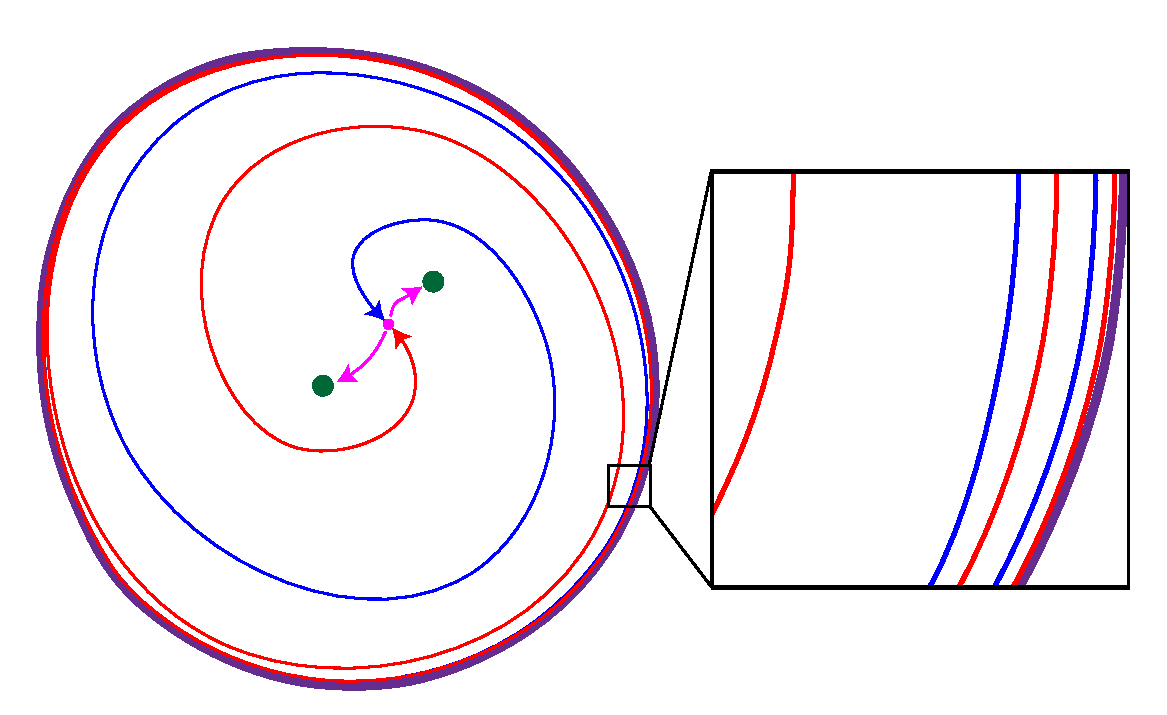
\includegraphics[width=0.5\textwidth]{unstab_lc_3fps}
  \caption{Separatrix between two stable fixed points inside an unstable limit cycle.
  }\label{fig:unstab_lc_3fps}
\end{SCfigure}



\subsection{Perturbing limit cycles}
If the limit cycle is hyperbolic, the Hausdorff distance between the original and perturbed limit cycles tends to scale linearly with \(\epsilon\), the size of the perturbation. That is,

\[
d_H(\gamma_0, \gamma_\epsilon) = O(\epsilon),
\]

where \(d_H\) denotes the Hausdorff distance. The linear dependence arises because small changes in the vector field result in small changes in the trajectories of the system, which leads to a nearby limit cycle.


\subsubsection{Period closeness}\label{sec:periodcloseness}
%TODO: 
\begin{proposition}\label{prop:periodcloseness}%For a limit cycle from
Take a vector field $f\in C^1$.
If $\dot x = f(x)$ has a hyperbolic limit cycle with period $T_f$ then there is $\epsilon$ for which all $g$ in a $\epsilon$ $C^1$ neighbourhood will have a limit cycle (with the same stability) with period $T_g$ such that  $|T_f-T_g| = \mathcal{O}(\epsilon)$.
\end{proposition}

\begin{proof}
Existence and Hausdorff distance of $\mathcal{O}(\epsilon)$ follows from PMT.
Parametrize the limit cycle orbit by $\theta$.
Then $T_f = \frac{1}{\int_{\theta=0}^{2\pi}f(\gamma_f(\theta))d\theta}$.
There if a $k\in\reals$ such that $\gamma_{\text{Arc Length}} - \gamma_{\text{Arc Length}}<k\epsilon$.

\[\text{Arc Length} = \int_a^b \sqrt{1 + [f'(x)]^2} \, dx.\]
%\begin{align}
%\int_{\gamma_f}\sqrt{1 + [f(x)]^2}dx\\
%\int_{\gamma_g}\sqrt{1 + [g(x)]^2}dx
%\end{align}

$\gamma_f(\theta)-\gamma_g(\theta) = \mathcal{O}(\epsilon) \leq m\epsilon$ %use homeomorphism for mapping! from PMT


USE LIPSCHITZ! 
$\|f(x)-f(y)\|\leq L_f\|x-y\|$
$\|g(x)-g(y)\|\leq L_g\|x-y\|$


\begin{align}
f(\gamma_f(\theta)) - g(\gamma_g(\theta)) \leq  L_fL_gm\epsilon.
\end{align}

So \[\int_{\theta=0}^{2\pi}f(\gamma_f(\theta))d\theta-g(\gamma_g(\theta))d\theta\leq L_fL_gm\epsilon\theta.\]


Use Davis-Kahan theorem. 
This states that the largest eigenvalues (0 for a stable limit cycle) are at most 
\end{proof}


\begin{theorem}[Davis-Kahan]
Let \( A \) and \( B \) be \( n \times n \) Hermitian matrices with eigenvalues \( \lambda_1 \leq \lambda_2 \leq \dots \leq \lambda_n \) for \( A \), and \( \mu_1 \leq \mu_2 \leq \dots \leq \mu_n \) for \( B \). Let \( \Delta = A - B \), and let \( \delta = \| \Delta \| \) be the operator norm of \( \Delta \). Then, for any eigenvalue \( \lambda_i \) of \( A \) and \( \mu_j \) of \( B \), the Davis-Kahan theorem gives the following bound on the difference between the eigenvalues of \( A \) and \( B \):
\[
|\lambda_i - \mu_i| \leq \frac{\| \Delta \|}{\sin \theta_i}
\]
where \( \theta_i \) is the angle between the eigenvectors corresponding to \( \lambda_i \) and \( \mu_i \). That is, if \( v_i \) is the eigenvector of \( A \) corresponding to \( \lambda_i \) and \( w_i \) is the eigenvector of \( B \) corresponding to \( \mu_i \), then
\[
\cos \theta_i = | \langle v_i, w_i \rangle |.
\]
\end{theorem}

For a discussion and proofs of this theorem see for example Section V.3 of \citet{stewart1990matrix}.


\begin{theorem}[Wedin's Theorem]
Let \( A \in \mathbb{C}^{m \times n} \) and \( \tilde{A} \in \mathbb{C}^{m \times n} \) be two matrices such that \( \| A - \tilde{A} \| \) is small, where \( \| \cdot \| \) denotes a matrix norm. Then, for the singular values \( \sigma_i(A) \) and \( \sigma_i(\tilde{A}) \), and corresponding singular vectors \( \mathbf{u}_i(A) \), \( \mathbf{v}_i(A) \), \( \mathbf{u}_i(\tilde{A}) \), \( \mathbf{v}_i(\tilde{A}) \), the following bounds hold:
\[
\left| \sigma_i(A) - \sigma_i(\tilde{A}) \right| \leq \| A - \tilde{A} \| \cdot \max_{j \neq i} \frac{\sigma_j(A)}{\sigma_i(A)}
\]
and for the singular vectors:
\[
\| \mathbf{u}_i(A) - \mathbf{u}_i(\tilde{A}) \| \leq \frac{\| A - \tilde{A} \|}{\sigma_i(A)} \cdot \max_{j \neq i} \frac{\sigma_j(A)}{\sigma_i(A)}
\]
\[
\| \mathbf{v}_i(A) - \mathbf{v}_i(\tilde{A}) \| \leq \frac{\| A - \tilde{A} \|}{\sigma_i(A)} \cdot \max_{j \neq i} \frac{\sigma_j(A)}{\sigma_i(A)}
\]
\end{theorem}



\subsubsection{Period matching}
%obsolete?
\subsubsection{Applying Melnikov’s Method to Limit Cycles}

To understand the period change due to a perturbation of a limit cycle, let’s consider the following:

Suppose we have an unperturbed system
\[
\dot{x} = f(x)
\]
with a limit cycle \(\gamma_0\) of period \(T_0\).

Now we apply a small perturbation to the system:
\[
\dot{x} = f(x) + \epsilon g(x),
\]
where \(g(x)\) represents the perturbation, and \(\epsilon\) is a small parameter.

The Melnikov function \(M(t)\) measures the first-order effect of the perturbation on the limit cycle, and it is given by:
\[
M(t) = \int_0^{T_0} \langle \nabla H(x_0(t)), g(x_0(t)) \rangle \, dt,
\]
where:
\begin{itemize}
    \item \(x_0(t)\) is the trajectory along the limit cycle \(\gamma_0\),
    \item \(H(x)\) is the Hamiltonian (or energy function) associated with the unperturbed system,
    \item \(g(x)\) is the perturbation vector field,
    \item \(\langle \cdot, \cdot \rangle\) denotes the dot product.
\end{itemize}

The Melnikov function tells us how the perturbation influences the distance between stable and unstable manifolds in the phase space. It is closely related to the splitting of separatrices, but in the context of limit cycles, it helps predict changes in the period and persistence of the limit cycle.

For small perturbations:

\(M(\gamma_0)\) represents the sensitivity of the period or structure of the limit cycle to the perturbation.

If \(M(\gamma_0) \neq 0\), the limit cycle may shift slightly, but it will persist, and the change in the period can be approximated as:
\[
\Delta T \approx \epsilon M(\gamma_0),
\]
meaning that the period change is proportional to \(\epsilon\), the size of the perturbation, with \(M(\gamma_0)\) determining the proportionality constant.

If \(M(\gamma_0) = 0\), the system is at a critical point where a bifurcation may occur, and the limit cycle may undergo a qualitative change (e.g., it could disappear or bifurcate).



\subsubsection{Homeomorphism and homotopy}

A homeomorphism \( f \) between the two limit cycles is a continuous, bijective map that transforms points on \( \gamma_1(t) \) to points on \( \gamma_2(s) \) while preserving the topological structure. Mathematically, this is expressed as:
\[
f: \gamma_1(t) \rightarrow \gamma_2(s), \quad \text{where} \quad s = h(t)
\]
Here, \( h(t) \) is a continuous, bijective, and periodic function that maps the time variable \( t \) in System 1 to the time variable \( s \) in System 2, i.e.,
\[
h: [0, T_1] \rightarrow [0, T_2]
\]
with the condition that \( h(0) = 0 \) and \( h(T_1) = T_2 \).

The map \( f \) in terms of the coordinates can be written as:
\[
f(x_1(t), y_1(t)) = (x_2(h(t)), y_2(h(t)))
\]



The homotopy \( H \) between two limit cycles \( \gamma_1(t) \) and \( \gamma_2(t) \) is expressed as:
\[
H: [0,1] \times [0, T] \rightarrow \mathbb{R}^n
\]
where \( H(\tau, t) \) gives the position of a point on the limit cycle at time \( t \) and for a given \( \tau \). The transformation satisfies:
\[
H(0, t) = \gamma_1(t), \quad H(1, t) = \gamma_2(t)
\]
This means that at \( \tau = 0 \), the homotopy corresponds to the first limit cycle \( \gamma_1 \), and at \( \tau = 1 \), the homotopy corresponds to the second limit cycle \( \gamma_2 \). For intermediate values of \( \tau \), \( H(\tau, t) \) represents a continuous deformation between \( \gamma_1 \) and \( \gamma_2 \).



\subsection{Non-autonomous}
\subsubsection{Asymptotically autonomous dynamical systems}
\citep{wieczorek2021compactification}


\end{document}
